
\documentclass{article}

% Recommended, but optional, packages for figures and better typesetting:
\usepackage{microtype}
\usepackage{graphicx}
% \usepackage{subfigure}
\usepackage{subcaption} 
\usepackage{booktabs} % for professional tables

\usepackage{url}
\usepackage{enumitem} 
\usepackage{tabularx} 
\usepackage{centernot}
\usepackage[parfill]{parskip}
\usepackage{quiver}
\usepackage{bbm} 
\usepackage{graphicx} 
\usepackage{scalerel}
\usepackage{nicefrac} 
\usepackage{bbm} 

% hyperref makes hyperlinks in the resulting PDF.
% If your build breaks (sometimes temporarily if a hyperlink spans a page)
% please comment out the following usepackage line and replace
% \usepackage{icml2024} with \usepackage[nohyperref]{icml2024} above.
\usepackage{hyperref}


% Attempt to make hyperref and algorithmic work together better:
\newcommand{\theHalgorithm}{\arabic{algorithm}}

% Use the following line for the initial blind version submitted for review:
\usepackage{icml2024}

% If accepted, instead use the following line for the camera-ready submission:
% \usepackage[accepted]{icml2024}

% For theorems and such
\usepackage{amsmath}
\usepackage{amssymb}
\usepackage{mathtools}
\usepackage{amsthm}

% if you use cleveref..
\usepackage[capitalize,noabbrev]{cleveref}

%%%%%%%%%%%%%%%%%%%%%%%%%%%%%%%%
% THEOREMS
%%%%%%%%%%%%%%%%%%%%%%%%%%%%%%%%
\theoremstyle{plain}
\newtheorem{theorem}{Theorem}[section]
\newtheorem{proposition}[theorem]{Proposition}
\newtheorem{lemma}[theorem]{Lemma}
\newtheorem{corollary}[theorem]{Corollary}
\theoremstyle{definition}
\newtheorem{definition}[theorem]{Definition}
\newtheorem{assumption}[theorem]{Assumption}
\theoremstyle{remark}
\newtheorem{remark}[theorem]{Remark}
\theoremstyle{remark} 
\newtheorem{example}[theorem]{Example} 

% Todonotes is useful during development; simply uncomment the next line
%    and comment out the line below the next line to turn off comments
%\usepackage[disable,textsize=tiny]{todonotes}
\usepackage[textsize=tiny]{todonotes}


% The \icmltitle you define below is probably too long as a header.
% Therefore, a short form for the running title is supplied here:
\icmltitlerunning{Submission and Formatting Instructions for ICML 2024}

\begin{document}

\twocolumn[
\icmltitle{Analyzing GFlowNets: Limitations, Countermeasures, and Assessment}

% It is OKAY to include author information, even for blind
% submissions: the style file will automatically remove it for you
% unless you've provided the [accepted] option to the icml2024
% package.

% List of affiliations: The first argument should be a (short)
% identifier you will use later to specify author affiliations
% Academic affiliations should list Department, University, City, Region, Country
% Industry affiliations should list Company, City, Region, Country

% You can specify symbols, otherwise they are numbered in order.
% Ideally, you should not use this facility. Affiliations will be numbered
% in order of appearance and this is the preferred way.
\icmlsetsymbol{equal}{*}

\begin{icmlauthorlist}
\icmlauthor{Firstname1 Lastname1}{equal,yyy}
\icmlauthor{Firstname2 Lastname2}{equal,yyy,comp}
\icmlauthor{Firstname3 Lastname3}{comp}
\icmlauthor{Firstname4 Lastname4}{sch}
\icmlauthor{Firstname5 Lastname5}{yyy}
\icmlauthor{Firstname6 Lastname6}{sch,yyy,comp}
\icmlauthor{Firstname7 Lastname7}{comp}
%\icmlauthor{}{sch}
\icmlauthor{Firstname8 Lastname8}{sch}
\icmlauthor{Firstname8 Lastname8}{yyy,comp}
%\icmlauthor{}{sch}
%\icmlauthor{}{sch}
\end{icmlauthorlist}

\icmlaffiliation{yyy}{Department of XXX, University of YYY, Location, Country}
\icmlaffiliation{comp}{Company Name, Location, Country}
\icmlaffiliation{sch}{School of ZZZ, Institute of WWW, Location, Country}

\icmlcorrespondingauthor{Firstname1 Lastname1}{first1.last1@xxx.edu}
\icmlcorrespondingauthor{Firstname2 Lastname2}{first2.last2@www.uk}

% You may provide any keywords that you
% find helpful for describing your paper; these are used to populate
% the "keywords" metadata in the PDF but will not be shown in the document
\icmlkeywords{Machine Learning, ICML}

\vskip 0.3in
]

% this must go after the closing bracket ] following \twocolumn[ ...

% This command actually creates the footnote in the first column
% listing the affiliations and the copyright notice.
% The command takes one argument, which is text to display at the start of the footnote.
% The \icmlEqualContribution command is standard text for equal contribution.
% Remove it (just {}) if you do not need this facility.

%\printAffiliationsAndNotice{}  % leave blank if no need to mention equal contribution
\printAffiliationsAndNotice{\icmlEqualContribution} % otherwise use the standard text.

\begin{abstract}
Generative Flow Networks (GFlowNets) are powerful samplers for distributions over compositional objects (e.g., graphs). Despite their increasing popularity, GFlowNets are still in their infancy, and many fundamental questions about them remain unexplored. In this work, we analyze GFlowNets from three fundamental perspectives: expressiveness, stability, and model evaluation.  


Regarding expressiveness, we consider GFlowNets for graph generation. We prove that, given a suitable state graph, GFlowNets can accurately learn any distribution supported over trees. Strikingly, however, we show simple combinations of state graphs and reward functions that cause GFlowNets to fail --- i.e., for which balance is unattainable. We propose leveraging embeddings of children's states to circumvent this limitation and thus increase the expressiveness of GFlowNets, provably.

For stability, we analyze tree-structured state graphs and discuss how fluctuations in balance conditions impact the accuracy of GFlowNets, i.e., the gap between the sampling and target distributions. Our theoretical results suggest that i) flow imbalances near the initial state have a higher impact than those near terminal ones; ii) imbalance in a single edge may be catastrophically propagated within the state graph, severely damaging the approximation to the target distribution.

Finally, we revisit evaluation procedures for GFlowNets and highlight the pitfalls of broadly used procedures. We provide guidelines for a more reliable evaluation of GFlowNets.


\end{abstract}

\section{Introduction} 

We contribute by 

\begin{enumerate} 
    \item providing flow-based bounds on the total variation distance between the target distribution and the distribution learned by a GFlowNet (\autoref{sec:flows}); % . 
    \item establishing the distributional limits of GFlowNets with GNN-based forward policies and showing that using a non-inductively biased neural network significantly hinders training convergence due to an exponential  increase in the state graph's size (\autoref{sec:rep}); 
    \item designing efficient and robust diagnostics for assessing the training convergence of GFlowNets (\autoref{sec:cov}); 
    \item rigorously comparing, through the proposed diagnostics, the rate of convergence induced by each of the previously proposed training objectives for GFlowNets in a comprehensive set of experiments (\autoref{sec:experiments}).        
\end{enumerate} 

\newpage 
% a
% \newpage 


\section{Background and related works} 

\paragraph{Notations and definitions.} Let $\mathcal{X}$ be a finite set and $\tilde{\pi}$ be a (possibly) unnormalized distribution over $\mathcal{X}$ with \textit{partition function} $Z = \sum_{x \in \mathcal{X}} \tilde{\pi}(x)$. Moreover, let $\mathcal{S} \supseteq \mathcal{X}$ be an extension of $\mathcal{X}$ and $\mathcal{G} = (\mathcal{S}, \mathbf{A})$ be a DAG over $\mathcal{S}$ with adjacency matrix $\mathbf{A} \in \{1, 0\}^{|\mathcal{S}| \times |\mathcal{S}|}$. We call the elements of $\mathcal{S}$ \textit{states} and assume the existence of a detached state, $s_{o}$, named the \textit{initial state}, which has no incoming edges and from which every other $v \in \mathcal{S}$ is reachable; $\mathcal{G}$ is then called the \textit{state graph} and the elements $x \in \mathcal{X}$, which assumedly have no outgoing edges, are called \textit{terminal states}. In this setting, we define a \textit{flow} over $\mathcal{G}$ as a function $F \colon \mathcal{S} \times \mathcal{S} \rightarrow \mathbb{R}_{+}$ such that $F(u, v) > 0$ if $\mathbf{A}_{uv} = 1$ and $F(u, v) = 0$ otherwise. Similarly, we let the \textit{flow through a node} $v \in \mathcal{S} \setminus \mathcal{X}$, denoted by $F_{N}$, be the sum of flows within all $v$'s outgoing edges, i.e., $F_{N}(v) = \sum_{u \in V} \mathbf{A}_{vu} F(v, u)$; for $x \in \mathcal{X}$, we let $F_{N}(x) = \tilde{\pi}(x)$. In this context, a \textit{forward policy} $p_{F}$ over $\mathcal{G}$ is a flow such that the projection $u \mapsto p_{F}(v, u)$ is a probability distribution over $\mathcal{S}$ for each $v \in \mathcal{S}$. On the other hand, a \textit{backward policy} $p_{B}$ over $\mathcal{G}$ is a forward policy over $\mathcal{G}^{\intercal} = (\mathcal{S}, \mathbf{A}^{\intercal})$. In both cases, note that a policy defines a conditional distribution over the trajectories $\tau = (s_{i})_{i=0}^{M}$ in $\mathcal{G}$ by $p_{F}(\tau | s_{o}) = \prod_{i=1}^{M} p_{F}(s_{i - 1}, s_{i})$ and that it is related to the edge-level flow $F$ by $F(u, v) = p_{F}(u, v) F_{N}(u)$.  

\paragraph{GFlowNets.} A \textit{GFlowNet} is represented as a tuple $(\log p_{F}(\cdot ; \theta_{F}), \log p_{B}(\cdot ; \theta_{B}), \log F_{N}(\cdot ; \theta_{N}), \theta_{\log Z})$ consisting of parametric models for the forward and backward policies and sometimes for flow $\log F_{N}$ and the partition function's logarithm $\theta_{\log Z}$ (when such quantities are not estimated, we simply let $\theta_{N} = \theta_{\log Z} = \emptyset$). Importantly, the unknown functions $\log p_{F}$, $\log p_{B}$ and $\log F_{N}$ are parameterized by neural networks and are trained to ensure that the marginal distribution of $p_{F}$ over $\mathcal{X}$, 
\begin{equation} \label{eq:marg} 
    p_{\intercal}(x ; \theta_{F}) \coloneqq \sum_{\tau \rightsquigarrow x} p_{F}(\tau | s_{o} ; \theta_{F}),  
\end{equation}
matches the normalized target distribution $\pi(x) = \tilde{\pi}(x) / Z$ for each $x \in \mathcal{X}$. Notoriously, contrasting with MCMC-based methods, the quantity $p_{\intercal}(x ; \theta_{F})$ may be unbiasedly estimated by an importance sampling estimator based on $p_{B}$ as a proposal distribution, which we denote by $\hat{p}_{\intercal}$. 

% A GFlowNet is a model parameterized in many distinct ways with allegedly purposeful distributional guarantees. 

\paragraph{Training GFlowNets.} \autoref{eq:marg} sums over a potentially intractable number of terms and it is generally not possible to directly minimize a difference between $p_{\intercal}$ and $\pi$ to estimate the parameters of a GFlowNet. Consequently, the training of GFlowNets is based upon the enforcement of trajectory-level \textit{balance conditions} ensuring that $p_{\intercal} = \pi$; Bengio, for instance, originally proposed the \textit{flow-matching} condition guaranteeing that the flows entering and leaving a state $v \in \mathcal{S}$ are the same, namely, 
\begin{equation}
    \sum_{u \in \mathcal{S}} \mathbf{A}_{uv} F(u, v) = \sum_{w \in \mathcal{S}} \mathbf{A}_{vw} F(v, w) + \mathbbm{1}_{v \in \mathcal{X}} \tilde{\pi}(v),   
\end{equation}
which they proved sufficient for $p_{\intercal} = \pi$ and was practically enforced by the minimization of the expected squared log-ratio between its left- and right-hand sides under a distribution with full-support over $\mathcal{S}$. Nonetheless, enumerating the parents and children of a state is a computationally burdensome endeavor and the flow-matching condition is not a practically useful training objective for GFlowNets; this observation led to the development of alternative and easy-to-verify balance conditions. More specifically, let $\tau = (s_{i})_{i=0}^{M}$ be a trajectory in $\mathcal{G}$ and, for $0 \le m < n \le M$,  
\begin{equation} \label{eq:stbalance}  
    \mathcal{L}_{m, n}(\tau) = \left( \log \frac{F(s_{m}) \prod_{i = m + 1}^{n} p_{F}(s_{i - 1}, s_{i})}{F(s_{n}) \prod_{i = m + 1}^{n} p_{B}(s_{i}, s_{i - 1})} \right)^{2},  % . 
\end{equation}
in which we omitted the dependency of $\mathcal{L}_{m, n}$ on the parameters of $p_{F}$, $p_{B}$ and $F$ for clarity; we further assume that $\log F(s_{o}) = \theta_{\log Z}$ and $F(x) = \tilde{\pi}(x)$ for each $x \in \mathcal{X}$. Then, the \textit{trajectory balance} (TB) objective is defined by $\mathcal{L}_{TB}(\tau) \coloneqq \mathcal{L}_{o, M}(\tau)$. Correspondingly, the \textit{detailed balance} (DB) objective is $\mathcal{L}_{DB}(\tau) = \sum_{m=1}^{M} \mathcal{L}_{m - 1, m}(\tau)$. Finally, the \textit{subtrajectory balance} (SubTB) objective is, for a hyperparameter $\lambda \in [0, 1]$, determined by   
\begin{equation}
    \mathcal{L}_{SubTB}(\tau) = \frac{\sum_{0 \le m < n \le M} \lambda^{n - m} \mathcal{L}_{m, n}(\tau)}{\sum_{0 \le m < n \le M} \lambda^{n - m}}; 
\end{equation}
in practice, $\lambda$ is commonly fixed at $.9$. Notably, it is currently unclear how a deviance from satisfying a balance condition, which is defined within an extension of the target distribution $\pi$'s support, relates to the discrepancy between GFlowNet's marginal distribution $p_{\intercal}$ and $\pi$. Our work is the first step towards  understanding this relationship.  

% Then, the \textit{trajectory balance} condition is defined by $\mathcal{L}_{TB}(\tau) = \mathcal{L}_{0 M} $ 

% we further assume that $F(s_{o}) = \theta_{\log Z}$ and $F(x) = \tilde{\pi}(x)$ for each $x \in \mathcal{X}$. 
% Consequently, the training of GFlowNets is based upon trajectory-level \textit{balance conditions}.  

% Expose the different training objectives for GFlowNets and their different parameterizations 

\paragraph{Diagnosing GFlowNets.} Assessing the goodness-of-fit of a trained GFlowNet is an important problem mostly unaddressed by the literature. Indeed, previous works considered measures such as the average unnormalized target, $\mathbb{E}_{x \sim p_{\intercal}}[\tilde{\pi}(x)]$, and (Pearson) correlation between the $\log p_{\intercal}$ and $\log \tilde{\pi}$, both of which fail by attributing a respectively high or perfect scores to an incorrectly learned $p_{\intercal} \propto \tilde{\pi}^{\alpha}$ for $\alpha > 1$; the \textit{accuracy} of a GFlowNet, defined by 
\begin{equation}
    \min \left\{ \frac{\mathbb{E}_{x \sim p_{\intercal}}\left[ \tilde{\pi}(x) \right]}{\mathbb{E}_{x \sim \pi} \left[ \tilde{\pi}(x) \right]}, 1 \right\}, 
\end{equation}
similarly assigns an inappropriately high value to a learned distribution with excessive probability mass on the target's modes. Alternatively, when the target distribution support's $\mathcal{X}$ is small enough to be enumerated, one may directly compare $\tilde{\pi}$ to $p_{\intercal}$; however, $\mathcal{X}$ is generally very large and this approach is generally unfeasible. In this setting, our work is the first to consider general and correct diagnostics for GFlowNets and to use them to extensively compare the efficacy of previously proposed training objectives.  


\textcolor{red}{\bf If G1 and G2 have loss(G1) < loss (G2), can l1(G1) > l2(G2)?}

% In this scenario, our work is the first to design efficient and correct diagnostics and to fairly compare the GFlowNets' training objectives. 

% In this scenario, our work is the first to propose provably correct and efficiently implementable diagnostic procedures and to fairly 

% Using the unbiased estimator may be a good starting diagnostic (on a fixed heldout set)

% This will require a huge amount of work for subsuming a comprehensive theory 

\section{Flow-based deterministic bounds on the total variation of GFlowNets} \label{sec:flows} 

We start our analysis by quantifying the consequences of a deviance from the flows' balance on the underlying marginal distribution over the terminal states. Our results highlight, on the one hand, that a lack of flow-balance upstream in the generative process is more damaging to the overall distributional accuracy of a GFlowNet than an equivalent imbalance nearer the terminal states; on the other hand, that a disruption of the detailed balance condition in a single edge may be catastrophically propagated within the network and severely damage the approximation to the target distribution. See the appendix for self-contained proofs of our results. 

\begin{figure}[t]
    \center 
    \def\spacing{-15pt}
\[\begin{tikzcd}
	&[\spacing]&[\spacing] {F+\delta} \\
	&[\spacing] {\frac{F}{g}+\delta} &[\spacing]&[\spacing]&[\spacing] {\frac{F}{g}} \\
% 	& \triangle & \triangle && \triangle & \triangle \\
    {\frac{F}{g^h}+\delta_1} &[\spacing] {\frac{F}{g^h}+\delta_2} &[\spacing]&[\spacing] % {\frac{F}{g^h}+\delta_{g^{h-1}}} 
    &[\spacing] {\frac{F}{g^h}} &[\spacing] {\frac{F}{g^h}} % & {\frac{F}{g^h}}
    \arrow["{\text{degree g}}", swap, from=1-3, to=2-2]
	\arrow[from=1-3, to=2-5]
	\arrow[from=2-5, to=3-6]
	\arrow[from=2-5, to=3-5]
	\arrow[from=2-2, to=3-1]
	\arrow[from=2-2, to=3-2] 
    % \arrow[from=3-2, to=4-1]
	% \arrow[from=3-2, to=4-2]
	% \arrow[from=3-3, to=4-3]
	% \arrow[from=3-5, to=4-5]
	% \arrow[from=3-6, to=4-6]
	% \arrow[from=3-6, to=4-7]
\end{tikzcd}\]
\caption{\textbf{Imbalanced flows in a regular tree} with width $g = 2$ and depth $h = 2$. The extra flow within the root's left child breaks the expected uniform distribution over the $g^{h}$ leaves.}
% \caption{\textbf{Imbalanced flow network in a tree.}}
% \caption{A flow network with a extra flow of $\delta$ in one of the branches of the initial state} 
    \label{fig:a} 
    % \label{fig:treesgraphs} 
\end{figure}

% \begin{theorem}[Total variation of the sampling distribution] Let $\delta >0$ and $\sum_{i=1}^{g^{h-1}} \delta_i = \delta$, where $\delta_i \in [0, \delta]$ for all $i \in \{1,2, \dots, g^{h-1}\}$. Suppose that we have the flow network $(G_T, F+\delta)$ abiding by Assumption~\ref{as: gf_tree_unif} besides the first edge from the root to a son where it has a $\delta$ increasing generating a new target distribution $\pi$ (see Figure [ref]).  Under these conditions, the total variation distance between $\pi$ and $\pi^*$ is bounded above and below by 
% \begin{align*}
% & \epsilon(\delta, g) \leq ||\pi - \pi^*||_{\scaleto{\textbf{TV}}{3pt}} \leq \epsilon(\delta, g^h) \quad \text{where}
% \\
% & \epsilon(a,b) := \Big(1 - \frac{1}{b} \Big) \frac{a}{F+a}\,.
% \end{align*}
% \end{theorem}


\paragraph{Bounds on TV for arbitrary state graphs.} We show that the intuition built upon the previous discussion relatively to tree-structured state graphs carries out to general acyclic generative processes, namely, (i) that an imbalanced edge reaching many terminal states has a larger impact on the approximation to the target distribution than an imbalanced edge leading to comparably fewer terminal states; and (ii) the difficult of training a GFlowNet is an increasing function of the target distribution's support. To start with, \autoref{thm:wca} lays out a worst-case analysis of the propagated errors within a flow network and underlines point (ii) above. 

\begin{theorem}[Deterministic flow-based bounds for the TV in general graphs] \label{thm:wca} 
    Let $(\mathcal{G}, F, \tilde{\pi})$ be a imbalanced flow network defined on a DAG $\mathcal{G}$ and $\tilde{\pi}$ be an uniform distribution supported on a space with $n$ objects. Assume that, except for an edge $(u, v)$ in $\mathcal{G}$, i.e., $\mathbf{A}_{uv} = 1$, for which  
    \begin{equation}
        F(s) p_{F}(s, s') - F(s') p_{B}(s', s) = \delta 
    \end{equation}
    with $\delta \ge 0$, the network is balanced. Let $p_{\intercal}^{(\delta)}$ be the corresponding marginal distribution over $\mathcal{X}$ and $d$ be the number of reachable terminal states from state $v$. Then, 
    \begin{equation}
        \frac{\delta (n - d)}{2n (F + \delta)} \le \|p_{\intercal}^{(\delta)} - \pi\|_{\scaleto{\textbf{TV}}{3pt}} \le \frac{\delta (n - 1)}{2n (F + \delta)}, 
    \end{equation}
    in which $\pi \propto \tilde{\pi}$ and $F(s_{o}) = F + \delta$ is the total flow. 
\end{theorem}
% \begin{theorem}[Total variation of the sampling distribution] Let $(G_n, F)$ be a flow network which should generates a target distribution $\pi$ uniform in the number of final vertices. Suppose there exists an edge in $G_n$, that is $s \to s' \in \mathbb{A}$ such that
% \[  F(s)P_{F}(s' | s) - F(s')P_{B}(s|s') = \delta \,,\]
% where $\delta > 0$. Then we have that $(G_n, F)$ generates a probability distribution $\mu_{\delta}$ such that
% \begin{align*}
% & \frac{\delta(n - d)}{2n(F + \delta)} \le ||\mu_{\delta} -\pi||_{\scaleto{\textbf{TV}}{3pt}} \leq \frac{\delta(n + dn - d)}{2n(F + \delta)} \,,
% \end{align*}
% where $d \in \{1,2, \dots, n-1\}$ is the number of final vertices that are descendants of $s'$. 
% \end{theorem}

Remarkably, this result shows that the accuracy of the downstream distribution depends linearly upon the deviation from the detailed balance within a single edge and, therefore, even a small error may lead to significant disruptions in the distributional approximation. Correspondingly, the result underscores the hardening properties of the number $n$ of terminal states regarding the training of GFlowNets: both the (provably tight) lower and upper bounds are increasing functions of $n$. Nonetheless, the preceding statement is poorly informative about the relevance of the particular imbalanced state to the overall generative process, an often observed phenomenon in worst-case analyses. In this context, we show in \autoref{thm:random} that, assuming Dirichlet-distributed downstream flows $\delta_{1}, \dots, \delta_{d}$ as shown in \autoref{fig:a} and an uniform target, the average TV distance between the learned and target distributions is an increasing function of the number of reachable states from the imbalanced node.  

\begin{theorem}[Expected TV under Dirichlet-distributed extra flows]\label{thm:random} 
    Let $(\mathcal{G}, F, \tilde{\pi})$ be the same imbalanced flow network as in \autoref{thm:wca}. Assume that the extra flow $\delta$ is distributed among the imbalanced node's terminal children according to a Dirichlet distribution with concentration parameter $\alpha \in \mathbb{R}^{d}$, i.e., 
    \begin{equation*}
        \left(\nicefrac{\delta_{i}}{\delta}\right)_{1 \le i \le d} \sim \textrm{Dir}\left(\alpha\right) % .   
    \end{equation*}
    (see \autoref{fig:a} for an illustration in trees). Denote $x_{i} = \nicefrac{\delta_{i}}{\delta} \in [0, 1]$ for $1 \le i \le d$ and $\mu_{\mathbf{x}, \delta}$ for the distribution resulted from the corresponding $\delta$-imbalance. Then, 
    \begin{equation*}
        \underset{\mathbf{x} \sim \textrm{Dir}(\alpha)}{\mathbb{E}} \left[ \|\mu_{\mathbf{x}, \delta} - \pi\|_{TV} \right] = \left( d \left( \Lambda - \frac{1}{n} \right) + 1 \right) \cdot \frac{\delta}{2(F + \delta)}, % .   
    \end{equation*}
    with, by letting $F_{a,  b}$ be the CDF of a $\textrm{Beta}(a, b)$ distribution,  
    \begin{equation*}
        \Lambda = \nicefrac{2}{n} F_{\alpha_{i}, 2\bar{\alpha}_{i}} \left( \nicefrac{1}{n} \right) - 2 F_{\alpha_{i} + 1, 2\bar{\alpha}_{i} + 1} \left( \nicefrac{1}{n} \right) + 1 - \nicefrac{1}{n} % . 
    \end{equation*}
    and $\bar{\alpha}_{i} = \sum_{j \neq i} \alpha_{j}$. 
\end{theorem}

However, it is unclear whether $\Lambda > \nicefrac{1}{n}$ and, in particular, whether $d$ positively or negatively influences the expected TV distance: for $n = 1$, $\Lambda = 0$, whereas $\lim_{n \rightarrow \infty} \Lambda = 1$. In this sense, \autoref{thm:random}'s corollary below reveals that, for uniformly distributed $\delta_{i}$, $d$ has a positive effect on the expected approximation error in all practically relevant cases, reiterating that ensuring the flow-balance in nodes from which many terminal states are reachable must be prioritized during training --- as we previously remarked in the context of tree-based state graphs. 

\begin{corollary} \label{col:random} 
    In \autoref{thm:random}, let $\alpha_{i} = 1$ for each $1 \le i \le d$, i.e., $(\nicefrac{\delta_{i}}{\delta})_{i=1}^{d}$ is uniformly distributed within the $(d + 1)$-dimensional simplex. Under these conditions, 
    \begin{equation*}
        \Lambda(d, n) = (d - 1) \left( \frac{1}{2} - \frac{1}{n} + \frac{1}{n^{2}}\right)  
    \end{equation*}
    and the expected TV between $\mu_{\mathbf{x}, \delta}$  and $\tilde{\pi}$, 
    \begin{equation*}
        \frac{\delta}{2(F + \delta)} \left( d \left( \Lambda(d, n) - \frac{1}{n} \right) + 1 \right),   
    \end{equation*}
    is an increasing function of $d \ge 1$ for $n > 2$. 
\end{corollary}
% Remarkably, this is very and very threatening to mankind and to the planet.  

% This is a weighted version of the detailed balance condition, which may be adequate for large state spaces under constraining computational settings

% \paragraph{Transition-decomposable and discriminatory DB loss ($\text{TD}^{3}$).}  

\paragraph{Theoretical analysis for tree-structured state graphs.} To gain some intuition, we first consider the scenario in which the state graph $\mathcal{G}$ is a regular tree with depth of $h$ in which each node, except the leaves representing the terminal states, has $g$ children and that the target distribution is uniform; see \autoref{fig:a}. Under these conditions, \autoref{thm:a} underscores that an improperly estimated flow near the initial state may significantly hinder the distributional approximation. 

\begin{example}[Total variation of the sampling distribution for trees] \label{thm:a} 
    Let $(\mathcal{G}, F, \tilde{\pi})$ be a balanced flow network with state graph $\mathcal{G}$ that is a tree with width $g$ and depth $h$, flow $F$ and uniform target distribution $\tilde{\pi}$.  Define $\delta \ge 0$ and $\sum_{i=1}^{g^{h - 1}} \delta_{i} = \delta$, with $\delta_{i} \in [0, \delta]$ for all $i \in \{1, 2, \dots, g^{h - 1}\}$. Then, assume that the flow within an edge stemming from the root has an increase of $\delta$, leading to an non-uniform marginal distribution $p_{\intercal}$ over the leaves; see \autoref{fig:a}. In this scenario, the total variation distance between $p^{\intercal}$ and $\pi \propto \tilde{\pi}$ is bounded above and below by 
    \begin{equation}
    \label{eq:a} 
    \begin{aligned}
        & \epsilon(\delta, g) \leq \|p_{\intercal} - \pi\|_{\scaleto{\textbf{TV}}{3pt}} \leq \epsilon(\delta, g^{h}), \, \text{with} \\ 
        & \epsilon(a, b) \coloneqq \left(1 - \frac{1}{b}\right) \frac{a}{F + a}.  
    \end{aligned}
    \end{equation} 
\end{example}

Notably, \autoref{eq:a} reveals that the effect of a broken balance of the learned flows over the downstream distribution crucially depends upon the height $h$ and, particularly, of the number of reachable leaves from the imbalanced edge; that is, the upper bound on the TV distance between $p_{\intercal}$ and $\pi$ increases exponentially in $h$ through $g^{h}$. Likewise, the lower bound on the TV increases as a function of the tree's width $g$, implying that the impact of the imbalance of the flows over $p_{\intercal}$ is larger for large state graphs than for comparably small ones. This underlines the advantages of building parsimonious state graphs and rigorously explains why the difficult of training a GFlowNet increases as we endeavor to approximate distributions with larger supports. 

\paragraph{Going beyond uniform distributions.} Our analysis was up to this moment based on the assumption of an uniform target distribution. Although insightful, this approach is somewhat constraining since a practitioner is generally interested in sampling from non-uniform distributions. In this context, \autoref{thm:app:a} in the appendix extends the previous results to multi-modal distributions and shows, similarly to \autoref{thm:a}, the relevance of upstream states and, differently from prior discussion, that the impact on the distributional accuracy of a lack of balance at a state having a large amount of probability mass concentrated among its descendants is larger than the impact corresponding to the imbalance of a state associated to a relatively small probability mass. This justifies, e.g., the empirical success of the replay buffer, which stores trajectories leading to high-probability terminal states and periodically replays them during training to reduce their associated error. 

% \paragraph{Transition-decomposable and discriminatory DB loss ($\text{TD}^{3}$).} 
\paragraph{Transition-decomposable discriminatory DB loss ($\text{TD}^{3}$).} \autoref{thm:a}, \autoref{thm:wca} and \autoref{thm:random} emphasized under different circumstances that, during training, one should prioritize ensuring the flow balance of states that are ancestral to high probability regions of the target distribution. Hence, we build upon this fact to define, for a trajectory $\tau = (s_{o}, s_{1}, \dots, s_{m})$, the loss function 
\begin{equation*}
    \mathcal{L}_{TD}(\tau) = \frac{1}{\sum_{i} \gamma(s_{i})} \sum_{1 \le i \le m} \gamma(s_{i}) \mathcal{L}_{i - 1, i}(\tau)% , 
\end{equation*}
(see \autoref{eq:stbalance}), in which $s \mapsto \gamma(s)$ is a weighting function; we call $\mathcal{L}_{TD}$ the \textit{transition-decomposable discriminatory detailed balance loss} ($\text{TD}^{3}$). Ideally, $\gamma(s)$ would be proportional to the probability mass associated with the $s$'s terminal descendants. In practice, however, it is very difficult to estimate such quantity in general state graphs and we instead consider $\gamma(s) = (T - d(s, s_{o}))^{2}$ as a proxy to this quantity, with $d(s, s_{o})$ as the geodesic distance between $s$ and the state graph's initial state and $T$ as the maximum trajectory length, which is always known. Intuitively, $\gamma$ assigns high weight to nodes upstream in the generative process leading to a large number of terminal states and, thus, related to a high probability region of the target. Moreover, we regard $\gamma$ as a quadratic function of $d(s, s_{o})$ (instead of a linear one) for the expected TV in \autoref{col:random} quadratically depends upon the imbalanced node's terminal children.   

% Moreover, we regard $\gamma$ as a quadratic function of $d(s, s_{o})$ as the expected TV in \autoref{col:random} quadratically depends upon the node's children.    

% Moreover, we regard $\gamma$ as a quadratic function of $d(s, s_{o})$ due to the quadratic dependence 

% Write about the annealing stuff (in the empirical section) and about using square instead of linear weighting 

\begin{figure}[!t] 
    \centering
    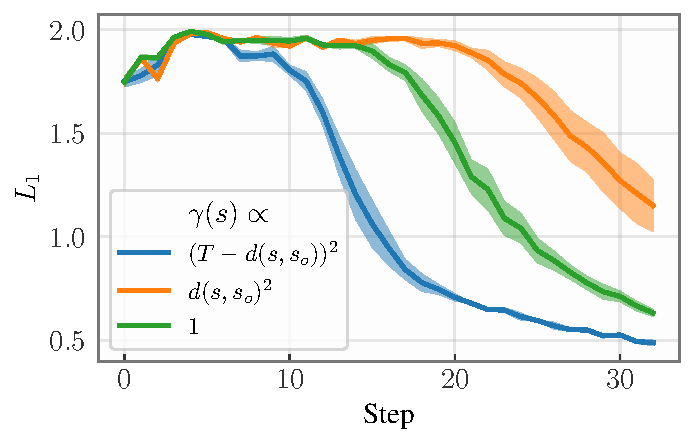
\includegraphics[width=.75\linewidth]{figures/avg_l1_gflownets_sets_weighted_db.pdf}
    \caption{\textbf{Weighted DB accelerates training convergence relatively to standard DB.} By weighting each transition proportionally to its closeness to the state graph's root, we notoriously improve upon the DB loss. This empirically supports our theoretical claims regarding the elevated importance of ensuring the balance within states leading to a large number of terminal states.}
    \label{fig:aaa}
\end{figure}

\paragraph{Empirical illustration.} 
We consider the task of generating discrete sets of fixed size with elements extracted from a finite warehouse; each element of this warehouse is assigned to a random positive value and the unnormalized distribution of a set corresponds to the product of its elements' values. 
% We consider the task of generating discrete sets of fixed size with elements extracted from a finite warehouse; each element of this warehouse is assigned to a random positive value and the unnormalized distribution of a set corresponds to the product of its elements' values. 
In this context, \autoref{fig:aaa} shows that $\mathcal{L}_{TD}$ significantly accelerates the training convergence of a GFlowNet relatively to a standard detailed balance loss (corresponding to setting $\gamma \coloneqq 1$), corroborating our rigorously laid analysis regarding the governing effect of imbalanced upstream states on the distributional approximation. Counterpositively, \autoref{fig:aaa} also points out that by weighting each transition proportionally to its distance to the root, thereby assigning larger weight to nodes downstream --- related to regions of relatively smaller probability ---, significantly worsens the resulting GFlowNet's accuracy. Notably, we found it beneficial to consider the tempered weighting function $\gamma_{\beta}(s) = \gamma(s)^{\beta}$ and linearly anneal the parameter $\beta$ to $0$ throughout training. We provide more implementation details in the accompanying supplementary material.  

% We provide more implementation details in the accompanying supplementary material.    

% This justifies, for instance, the empirical success of the replay buffer, a heuristics that consists of storing trajectories associated to high-probability terminal states and periodically replaying them during training to mitigate their deviation from balance.   

% \textcolor{red}{The results concerning multi-modal distributions in the appendix are very difficult to read and doesn't seem to be quite correct.} 

\newpage 

\section{Distributional limits of GNN-based policy networks} \label{sec:rep}  

\begin{figure}[!t] 
    \centering
    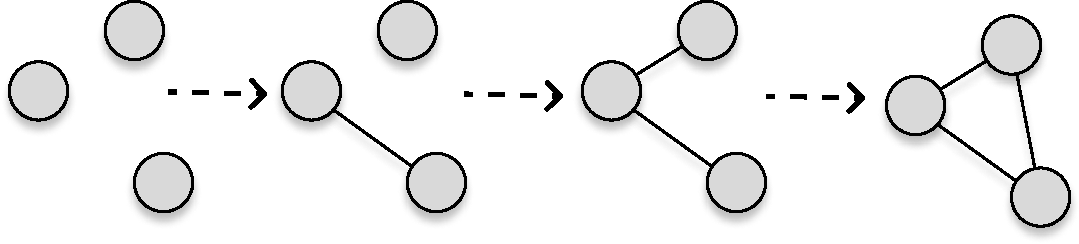
\includegraphics[page=1, width=\linewidth]{graphsss.pdf}
    \caption{\textbf{State graph for a GNN-based GFlowNet} generating 3-node graphs. The GNN's permutation invariance ensures each state is uniquely represented and the smallness resulting state graph.}% .}}
    \label{fig:gnns}
    \vspace{-12pt} 
\end{figure}

\paragraph{Advantages of GNN-based parameterizations.} By employing a GNN to parameterize the polices of a GFlowNet, one effectively reduces the size of the state graph $\mathcal{G}$ and significantly eases the optimization problem underlying the model's training, as was previously empirically observed by [ref]. Consider, for example, the generative process for graphs with three unlabeled nodes outlined in Figure [ref], in which we explicitly instantiate the state graph for a GFlowNet parameterized by a GNN (left) and by a neural network that is not permutationally invariant by design (right; e.g., an MLP). Noticeably, $\mathcal{G}$'s size is substantially reduced due to adoption of a permutation-invariant neural network: when generating graphs with $12$ nodes, for instance, this parameterization leads to a significant $5 \cdot 10^{13}$-fold reduction in $\mathcal{G}$'s size.  

\begin{figure}[!t] 
    \centering
    \includegraphics[page=2, width=\linewidth]{graphsss.pdf}
    \caption{\textbf{State graph for a MLP-based GFlowNet} generating 3-node graphs. The absence of an inductive bias for permutation variance leads to a different treatment for the column-wise isomorphic graphs by the MLP. Compare to \autoref{fig:gnns} and note the reduction in size due to using an inductively biased neural network. We omitted some edges from the state graph to avoid cluttering.} % .}}
    \label{fig:mlps}
\end{figure}

% Notably, by parameterizing the policies with a permutation-invariance task, the state graph's size for this task is reduced by a factorial  

% Notably, the state graph's size for this task factorially  

% Using a GNN to parameterize the distributions is very helpful. I am totally not motivated to continue writing this; the bounds of the preceding section are so, so, so loose, so damn loose. 

\begin{figure}
    \centering
    \begin{subfigure}{.49\linewidth}  
        \includegraphics[width=\textwidth]{figures/W&B Chart 1_7_2024, 10_25_46 PM.png}
        \caption{Heterogeneous target.}
    \end{subfigure}
    \begin{subfigure}{.49\linewidth} 
        \includegraphics[width=\textwidth]{figures/W&B Chart 1_7_2024, 10_26_45 PM.png}
        \caption{Homogeneous target.}
    \end{subfigure}
    \caption{\textbf{GNN-based GFlowNets are less expressive than their MLP-based counterparts.} GNN-based GFlowNets can learn to sample some (right), but not all (left), distributions represented by the state graph of \autoref{fig:gnns_state}. An MLP-based GFlowNet, in contrast, is not subject to such constraints and can sample from any target.}
    \label{fig:gnns}
\end{figure}

\paragraph{Limitations of 1-WL GNN-based parameterizations.} Nevertheless, despite its computational advantages, the use of GNN-based policies hinders the expressivity of GFlowNets due to the limited discriminative power of the 1-WL GNNs --- which are unable to distinguish some simple graph structures [ref]. 
Importantly, 1-WL GNNs such as GCN and GIN [ref, ref] are the most common GNN instances in practically used implementations of GFlowNets [ref, ref, ref].
In this context, the next theorem shows that there exist some distributions from which a GFlowNet parameterized by a GNN cannot learn to sample. 

\begin{figure}[!t] 
    \centering
    \includegraphics[page=3, width=\linewidth]{graphsss.pdf}
    \caption{\textbf{Limitations of a GNN-based GFlowNet.} The highlighted graphs are indistinguishable by a 1-WL GNN and, thus, a GFlowNet with such parameterization would learn the same policies at both states. Consequently, such GFlowNet cannot learn to sample from the target due to the heterogeneity of its unnormalized values at the root's left ($3$ and $3$) and right ($3$ and $5$) grandchildren.}
    \label{fig:gnns_state}
\end{figure}

\begin{theorem}[Distributional limits for GNN-based GFlowNets] 
\label{thm:aaa} 
    Let $(\mathcal{G}, p_{F}(\cdot ; \theta_{F}), p_{B}(\cdot ; \theta_{B}), F(\cdot ; \theta_{N}), \theta_{\log Z})$ be a GFlowNet and assume that $p_{F}$ is parameterized by a 1-WL GNN. Then, there is a state graph $\mathcal{G}$ and a target distribution $\tilde{\pi}$ such that there is no $\theta_{F}$ for which the learned marginal distribution matches $\pi \propto \tilde{\pi}$.   
\end{theorem}

Figure [ref] illustrates \autoref{thm:aaa}. As a 1-WL GNN cannot distinguish between the root's children, the GFlowNet will inevitably learn the same forward conditional distribution at both highlighted states. Thus, such GFlowNet is fundamentally unable to learn to sample from any distribution over the leaves in Figure [ref] in which the probabilities of the root's left and right grandchildren differ. 

\paragraph{Empirical illustration.} We validate our results in two different generative tasks. Firstly, Figure [ref] (left) shows that a GNN-based GFlowNet does converge substantially faster than an MLP-based one, both of which with approximately the same number of parameters, for the task of generating graphs with $n = 12$ unlabeled nodes. Secondly, Figure [ref] (right) confirms that, for the generative process depicted in Figure [ref], a GFlowNet employing GIN to parameterize the policies doesn't converge at all to the an heterogeneous target distribution; contrastingly, an MLP-based GFlowNet swiftly converges to the target distribution. The bottom line is that, when implementing GNNs to parameterize the GFlowNets' policies, one should be cautious to avoid limiting GFlowNet's capacity to learn to sample from the target distribution. This problem may be of particular concern in drug discovery --- in which non-insomorphic graphs indistinguishable by the 1-WL test may be commonly found. The discriminative power of GNNs, however, is not a constraining factor for causal discovery, where the sampled causal graphs' nodes are uniquely labeled and GNNs work as universal approximators, nor in phylogenetic inference, where the sampled complete binary trees that can be readily distinguished by the 1-WL test and, thus, by 1-WL GNNs. 

\textcolor{red}{Did the forward-looking trick work?}


\newpage

\section{Convergence diagnostics for GFlowNets} \label{sec:cov}  

In this section, we propose a provably correct metric for verifying the distributional incorrectness of GFlowNets, along with probably approximately correct (PAC) statistical guarantees for the accompanying estimators (\Cref{sec:assgfn}). Then, we apply this metric to two recently published methods for training GFlowNets, namely, LED- and FL-GFlowNets, and note that they are generally incapable of learning to sample from the target distribution (\Cref{sec:rev}). 

\subsection{Assessing GFlowNets} \label{sec:assgfn}

\paragraph{Flow Consistency in Sub-graphs (FCS).}  Let $(p_{F}, p_{B}, R)$ be a GFlowNet trained to sample from a distribution $R$ on $\mathcal{X}$. For each $x \in \mathcal{X}$, we can unbiasedly estimate the marginal probability of $x$ induced by $p_{F}$ through 
\begin{equation}
    p_{T}(x) = \sum_{\tau \rightsquigarrow x} p_{F}(\tau) = \mathbb{E}_{\tau \sim p_{B}(\cdot | x)} \left[ \frac{p_{F}(\tau)}{p_{B}(\tau)}  \right]. % ; % . 
\end{equation}
For frequently implemented benchmark environments for GFlowNets (such as grid world, sequence design and set generation), the preceding expectation may be directly computed by enumerating the (relatively small) trajectories leading to $x$. In this context, we build upon the identity 
\begin{equation}
    \mathbb{P}[X = x | X \in S] = \frac{\mathbb{P}[X = x]}{\mathbb{P}[X \in S]} = \frac{p_{T}(x)}{\sum_{y \in S} p_{T}(y)}  
\end{equation}
(and its analogous for $\pi = \nicefrac{R}{Z}$) for $X \sim  p_{T}$ and $S \subseteq \mathcal{X}$ to show that a correctly trained GFlowNet should satisfy the balance conditions in sub-graphs of the underlying flow network. For this, define for $S \subseteq \mathcal{X}$ 
\begin{equation*}
    \begin{split} 
    p_{T}^{(S)}(x ; \theta) = \frac{p_{T}(x ; \theta)}{\sum_{y \in S} p_{T}(y ; \theta)}, \, \pi^{(S)}(x) = \frac{R(x)}{\sum_{y \in S} R(y)} \\
    \text{ and } e(S, \theta) = \frac{1}{2} \sum_{x \in S} |p_{T}^{(S)}(x ; \theta) - \pi^{(S)}(x)|.
    \end{split} 
\end{equation*}
Finally, let $p$ be a distribution of full-support over fixed-size subsets of $\mathcal{X}$. In this scenario, the metric $\mathbb{E}_{S \sim p}[e(S, \theta)]$ quantifies GFlowNet's correctness in sub-graphs induced by $S \subseteq \mathcal{X}$; we call it the \emph{flow consistency in sub-graphs} (FCS). The following proposition shows that FCS is closely related to the TV distance between the learned and target distributions on $\mathcal{X}$. Nevertheless, contrarily to TV, FCS is computationally tractable since it is not reliant upon an extensive enumeration of the state graph. 

\begin{proposition}[Equivalence between TV and FCS] \label{prop:tv_fsc}  
    Let $p$ be a full-support distribution over $\{S \subseteq \mathcal{X} \colon |S| = B\}$ for some $B \ge 2$. Also, let $d_{TV} = e(\mathcal{X}, \theta)$ be the TV distance between $p_{T}$ and $\pi$ for a GFlowNet parameterized by $\theta$. Then, $d_{TV} = 0$ if and only if $\mathbb{E}_{S \sim p}[e(S, \theta)] = 0$.   
\end{proposition}


% Nevertheless, contrarily to TV, FCS does not require extensively searching the state graph.  


% $\{S_{1}, \dots, S_{N}\} \sim p$ be a random sample of fixed-size subsets of $\mathcal{X}$ according to a full-support distribution $p$. 

\paragraph{PAC statistical guarantees for $e(S ; \theta)$.} Realistically, we use a Monte Carlo approximation of the intractable quantity $\mathbb{E}_{S \sim p}[e(S, \theta)]$ to assess the accuracy of the learned GFlowNet due to the large size of $\mathcal{X}$. In this sense, the next proposition underlines that our estimator is, with high probability, a good approximation to FCS. % and, when learning is accurate, to TV. 

\begin{proposition}[PAC bound for FCS] \label{prop:pac} 
    Let $\{S_{1}, \dots, S_{m}\} \sim p$ be a random sample from the distribution $p$ of \Cref{prop:tv_fsc} and $\delta \in (0, 1)$. Then, 
    \begin{equation*}
        \begin{aligned} 
            \mathbb{P}_{S \sim p}\left[ 
                \underset{S \sim p}{\mathbb{E}} \left[ e(S, \theta) \right] 
                \le \frac{1}{m} \sum_{1 \le i \le m} e(S_{i}, \theta) + \sqrt{\frac{\log \frac{1}{\delta}}{2m}}    
            \right] \ge 1 - \delta.
        \end{aligned} 
    \end{equation*} 
    % and 
    % \begin{equation*}
    %     \begin{split} 
    %         \mathbb{P}_{S \sim p}\left[ d_{TV} \le \frac{1}{m} \sum_{1 \le i \le m} e(S_{i}, \theta) + s \right] \\
    %         \le \exp\left\{\left( d_{TV} - \mathbb{E}_{S \sim p} [ e(S, \theta) ]\right) + \frac{1}{8m} - s \right\}. 
    %     \end{split} 
    % \end{equation*}
\end{proposition}

This is, to the best of our knowledge, the first PAC-style result concerning GFlowNets. We believe that a rigorous analysis of the generalization capabilities of this class of models, which was already hinted by previous works [ref], will greatly benefit the understanding of its potentialities.   

\subsection{Revisiting LED- and FL-GFlowNets} \label{sec:rev} 

\paragraph{LED- and FL-GFlowNets.} 

\paragraph{Experimental setup.} 

\paragraph{Results.} 


% \paragraph{Using the the partition function's variance.} 

% \paragraph{Score-based goodness-of-fit test.} Use something similar to Stein's variational inference 

% \paragraph{Comparing the distribution of objects' features.} Exploit the compositionality of the sampled objects to compare the distributions of the samples' components  

\section{Experiments} \label{sec:experiments} 

\paragraph{Task descriptions.} 

\begin{enumerate}
    \item set generation, 
    \item design of sequences, 
    \item phylogenetic inference, 
    \item grid world, 
    \item linear preference learning, 
    \item bayesian structure learning 
\end{enumerate}

\paragraph{Experimental setup.} 

\paragraph{Comparing TB, SubTB, DB and CB.} 

% \section{Flows for trees and uniform distributions}


ping

\textcolor{blue}{
\textbf{To-do list (sensitivity analysis):}
\begin{enumerate}
    \item Sensitivity analysis for regular trees and uniform distribution 
    \item Generalization for DAGs
    \item Generalization for non-uniform distributions
\end{enumerate}
}
\textcolor{orange}{
\textbf{To-do list (policy networks):}
\begin{enumerate}
    \item Anonymous
    \begin{enumerate}
        \item Balance is impossible for some pairs of pointed DAGs and reward functions
        \item Some characterization of rewards that are particularly hard to approximate
        \item Sequences, Multisets, Anonymous and non-anonymous graphs (directed and undirected) 
\item trade-off between invariances in the networks and built into the state graph    \end{enumerate}
    \item Non-anonymous
\end{enumerate}
    }

\textcolor{red}{
\textbf{To-do list (evaluation and diagnostic of GFLowNets):}
\begin{enumerate}
    \item Current evaluation protocols are crap (usually focus on covering modes rather than approximation). Doing the right thing is also computationally infeasible for larges state-spaces 
    \item Convergence diagnostic based on some estimate of $\delta$, leveraging our theorems in the first part of the paper
    \item some diagonose based on, e.g, the estimates we can get from $R$ based on the trajectory-balance loss (in equilibrium, should be path independent, i.e., a constant)
\end{enumerate}
}

 

\section{Related works} 

\paragraph{Applications of GFlowNets.} 

\paragraph{Limitations of GNNs.} 

\section{Conclusions} 


\bibliographystyle{icml2024} 
\bibliography{bibliography} 

\newpage 
\onecolumn 

\appendix

\subsection{Uniform distributions and uniform flows}
\begin{itemize}
    \item A uniform flow of degree $g$ and height $h$ is a Markovian flow that models a uniform distribution, meaning all the leaf nodes have the same value. The policy of such flow consists in a function that takes the incoming flow and splits it equally between each of the g outgoing nodes.
\end{itemize}

To start let us consider the example of a flow trained on a uniform distribution and policy that takes the incoming flow and split it equally to all outgoing states. The resulting uniform distribution on the terminal nodes density is  represented by $\pi^*(x)=\frac{1}{g^h}$, for each terminal object in the domain $x \in \mathcal{X}$ and $|\mathcal{X}|=g^h$.

Let us consider the case that the policy at the root of the network introduces an error in the flow of size $\delta$, meaning that one children node now will receive a flow $\frac{F}{g}+\delta$ and the other $g-1$ will continue with $\frac{F}{g}$, which is equivalent to the policy with a probability density (after normalizing) that assigns a probability $\frac{F+g\delta}{g(F+\delta)}$ to one branch and $\frac{F}{g(F+\delta)}$ to the other $g-1$ branches. The total variation distance between this new density and the original policy (uniform probability for each $g$ branches) is $\epsilon(\delta, g)=(1-\frac{1}{g})\frac{\delta}{F+\delta}$. Now we denote the resulting sampling distribution induced by this modified flow as $\pi(x)$.


\begin{figure}[h]
    \center 
% https://q.uiver.app/#q=WzAsMTMsWzMsMCwiRitcXGRlbHRhIl0sWzIsMSwiXFxmcmFje0Z9e2d9K1xcZGVsdGEiXSxbNCwxLCJcXGZyYWN7Rn17Z31cXHRleHR7IH1cXHRyaWFuZ2xlIl0sWzIsMiwiXFx0cmlhbmdsZSJdLFswLDMsIlxcZnJhY3tGfXtnXmh9K1xcZGVsdGFfMSJdLFsxLDIsIlxcdHJpYW5nbGUiXSxbNSwyLCJcXHRyaWFuZ2xlIl0sWzQsMiwiXFx0cmlhbmdsZSJdLFsxLDMsIlxcZnJhY3tGfXtnXmh9K1xcZGVsdGFfMlxcdGV4dHsgIH1cXGxkb3RzICJdLFsyLDMsIlxcZnJhY3tGfXtnXmh9K1xcZGVsdGFfe2dee2gtMX19Il0sWzQsMywiXFxmcmFje0Z9e2deaH0iXSxbNSwzLCJcXGZyYWN7Rn17Z15ofSJdLFs2LDMsIlxcZnJhY3tGfXtnXmh9Il0sWzAsMSwiXFx0ZXh0e2RlZ3JlZSBnfSJdLFswLDJdLFsyLDZdLFsyLDddLFsxLDNdLFsxLDVdLFs1LDRdLFs1LDhdLFszLDldLFs3LDEwXSxbNiwxMV0sWzYsMTJdXQ==
\[\begin{tikzcd}
	&&& {F+\delta} \\
	&& {\frac{F}{g}+\delta} && {\frac{F}{g}\text{ }\triangle} \\
	& \triangle & \triangle && \triangle & \triangle \\
	{\frac{F}{g^h}+\delta_1} & {\frac{F}{g^h}+\delta_2\text{  }\ldots } & {\frac{F}{g^h}+\delta_{g^{h-1}}} && {\frac{F}{g^h}} & {\frac{F}{g^h}} & {\frac{F}{g^h}}
	\arrow["{\text{degree g}}", from=1-4, to=2-3]
	\arrow[from=1-4, to=2-5]
	\arrow[from=2-5, to=3-6]
	\arrow[from=2-5, to=3-5]
	\arrow[from=2-3, to=3-3]
	\arrow[from=2-3, to=3-2]
	\arrow[from=3-2, to=4-1]
	\arrow[from=3-2, to=4-2]
	\arrow[from=3-3, to=4-3]
	\arrow[from=3-5, to=4-5]
	\arrow[from=3-6, to=4-6]
	\arrow[from=3-6, to=4-7]
\end{tikzcd}\]
\caption{A flow network with a extra flow of $\delta$ in one of the branches of the initial state} 
    \label{fig:tree_graph} 
\end{figure}

Let $\mu$ and $\nu$ be two probability measures, then we denote $||\mu - \nu||_{\scaleto{\textbf{TV}}{3pt}}$ as the total variation distance between them. 

\begin{assumption}\label{as: gf_tree_unif}
 Let the pair $(G_T, F)$ be a flow network such that $G_T$ is a regular tree with degree $g$ and depth $h$. Furthermore, assume that $F$ spreads uniformly in the edges of $G_T$, then the target distribution $\pi^*$ generated by $(G_T, F)$ is uniform.      
\end{assumption}

\begin{theorem}[Total variation of the sampling distribution] Let $\delta >0$ and $\sum_{i=1}^{g^{h-1}} \delta_i = \delta$, where $\delta_i \in [0, \delta]$ for all $i \in \{1,2, \dots, g^{h-1}\}$. Suppose that we have the flow network $(G_T, F+\delta)$  abiding by Assumption~\ref{as: gf_tree_unif} besides the first edge from the root to a son where it has a $\delta$ increasing generating a new target distribution $\pi$. Then under these conditions describe the total variation distance between $\pi$ and $\pi^*$ is bounded above and below by the following
\begin{align*}
& \epsilon(\delta, g) \leq ||\pi - \pi^*||_{\scaleto{\textbf{TV}}{3pt}} \leq \epsilon(\delta, g^h) \quad \text{where}
\\
& \epsilon(a,b) := \Big(1 - \frac{1}{b} \Big) \frac{a}{F+a}\,.
\end{align*}
\end{theorem}

\begin{proof}
The terminal states of the modified flow network will have two types of nodes, with flow $\frac{F}{g^h}$ and $\frac{F}{g^h}+\delta_{i}$, with $\delta_i \geq 0$ and $\sum_{i=1}^{g^{h-1}} \delta_i = \delta$. We normalize those probabilities to obtain the individual probabilities for each terminal state, which determines the density of each sample. From that, we can proceed to compute the total variation distance between $\pi$ and $\pi^*$.
\begin{align*}
    ||\pi - \pi^*||_{\scaleto{\textbf{TV}}{3pt}} &= \frac{1}{2}\sum_{x \in \mathcal{X}} | \pi(x)- \pi^*(x) | \\
                          &= \frac{1}{2}\left[(g^h-g^{h-1})\left|\frac{F}{g^h}\frac{1}{F+\delta} - \frac{1}{g^h}\right|+ \sum_{i=1}^{g^{h-1}} \left|\frac{F+g^h\delta_i}{g^h}\frac{1}{F+\delta} - \frac{1}{g^h}\right| \right] \\
                          &= \frac{1}{2}\left[\frac{g^h\delta-g^{h-1}\delta+\sum_{i=1}^{g^{h-1}}|g^h\delta_i-\delta|}{g^h(F+\delta)}\right]
\end{align*}

We can lower bound $\sum_{i=1}^{g^{h-1}}|g^h\delta_i-\delta|$, by considering that $\sum_{i=1}^{g^{h-1}}(g^h\delta_i-\delta)=g^{h}\delta-g^{h-1}\delta$, taking the absolute value of the result and each element of the sum to obtain $g^{h}\delta-g^{h-1}\delta \leq \sum_{i=1}^{g^{h-1}}|g^h\delta_i-\delta|$. Thus we obtain the lower bound 
\begin{align*}
\frac{1}{2}\left[\frac{g^h\delta-g^{h-1}\delta+g^{h}\delta-g^{h-1}\delta}{g^h(F+\delta)}\right]&\leq \frac{1}{2}\left[\frac{g^h\delta-g^{h-1}\delta+\sum_{i=1}^{g^{h-1}}|g^h\delta_i-\delta|}{g^h(F+\delta)}\right] \\
                       \left(1-\frac{1}{g}\right)\frac{\delta}{F+\delta} &\leq  ||\pi - \pi^*||_{\scaleto{\textbf{TV}}{3pt}} 
\end{align*}.

This lower bound is reached when all error terms in the terminal states have the same value $\delta_i = \frac{\delta}{g^h}$.

To upper bound $|g^h\delta_i-\delta|$ we apply the triangle inequality, obtaining $|g^h\delta_i-\delta| \leq g^h\delta_i+\delta$ and  $\sum_{i=1}^{g^{h-1}}|g^h\delta_i-\delta| \leq g^h\delta+g^{h-1}\delta$, from which we obtain the upper bound
\begin{align*}
    ||\pi - \pi^*||_{\scaleto{\textbf{TV}}{3pt}} &\leq \frac{1}{2}\left[\frac{g^h\delta-g^{h-1}\delta + g^{h}\delta+g^{h-1}\delta}{g^h(F+\delta)}\right] \\
    ||\pi - \pi^*||_{\scaleto{\textbf{TV}}{3pt}} &\leq \frac{\delta}{F+\delta}
\end{align*}.

To obtain a tighter bound we break the sum $\sum_{i=1}^{g^{h-1}}|g^h\delta_i-\delta|$ by partitioning the sum into the first $I$ terms $S_A=g^h\sum_{i=1}^{I}|\delta_i-\frac{\delta}{g^h}|$ with $\delta_i < \frac{\delta}{g^h}$ and subsequent $g^{h-1}-I$ terms $S_B=g^h\sum_{j=I+1}^{g^{h-1}}|\delta_j-\frac{\delta}{g^h}|$ with $\delta_j \geq \frac{\delta}{g^h}$. By construction, we know that $S_A+g^h\sum_{i=1}^{I}\delta_i+g^h\sum_{j=I+1}^{g^{h-1}}\delta_j-S_B=g^{h-1}\delta$, simplifying to $S_B-S_A=\delta(g^h-g^{h-1})$. We rewrite $S_A + S_B = S_B-S_A+2S_A=\delta(g^h-g^{h-1})+2S_A$, and by triangle inequality on $S_A$, we obtain the upper bound $\sum_{i=1}^{g^{h-1}}|g^h\delta_i-\delta|=S_A+S_B \leq g^h\delta-g^{h-1}\delta+2I\delta $. Setting $I=g^{h-1}-1$ (the biggest value it can have without breaking the constraints on $\delta_i$), it simplifies to $S_A+S_B \leq g^h\delta+g^{h-1}\delta-2\delta $

\begin{align*}
    ||\pi - \pi^*||_{\scaleto{\textbf{TV}}{3pt}} &\leq \frac{1}{2}\left[\frac{g^h\delta-g^{h-1}\delta+\sum_{i=1}^{g^{h-1}}|g^h\delta_i-\delta|}{g^h(F+\delta)}\right] \\
    ||\pi - \pi^*||_{\scaleto{\textbf{TV}}{3pt}} &\leq \frac{1}{2}\left[\frac{g^h\delta-g^{h-1}\delta+g^h\delta+g^{h-1}\delta-2\delta }{g^h(F+\delta)}\right] \\
    ||\pi - \pi^*||_{\scaleto{\textbf{TV}}{3pt}} &\leq \left[\frac{g^h\delta-\delta }{g^h(F+\delta)}\right] \\
    ||\pi - \pi^*||_{\scaleto{\textbf{TV}}{3pt}} &\leq  \left(1-\frac{1}{g^h}\right)\frac{\delta}{F+\delta}
\end{align*}.
\end{proof}

\textcolor{red}{\begin{theorem}[Total variation of the sampling distribution] Let $\delta >0$ and $\sum_{i=1}^{n} \delta_i = \delta$, where $\delta_i \in [0, \delta]$. Suppose that we have the flow network $(G_n, F)$ which generates a target distribution $\pi^*$ uniform in the number of final vertices. Then if we increase the flow $F$ by $\delta$ in the same graph, that is $(G_n, F + \delta)$, generating a new target distribution $\pi$, the total variation distance between $\pi$ and $\pi^*$ is bounded above and below by the following
\begin{align*}
& ||\pi -\pi^*||_{\scaleto{\textbf{TV}}{3pt}} \leq \epsilon(\delta, n) \quad \text{where}
\\
& \epsilon(a,b) := \Big(1 - \frac{1}{b} \Big) \frac{a}{F+a}\,.
\end{align*}
\end{theorem}}




\section{Inherent limitations of policy networks}



\begin{figure}
    \center 
    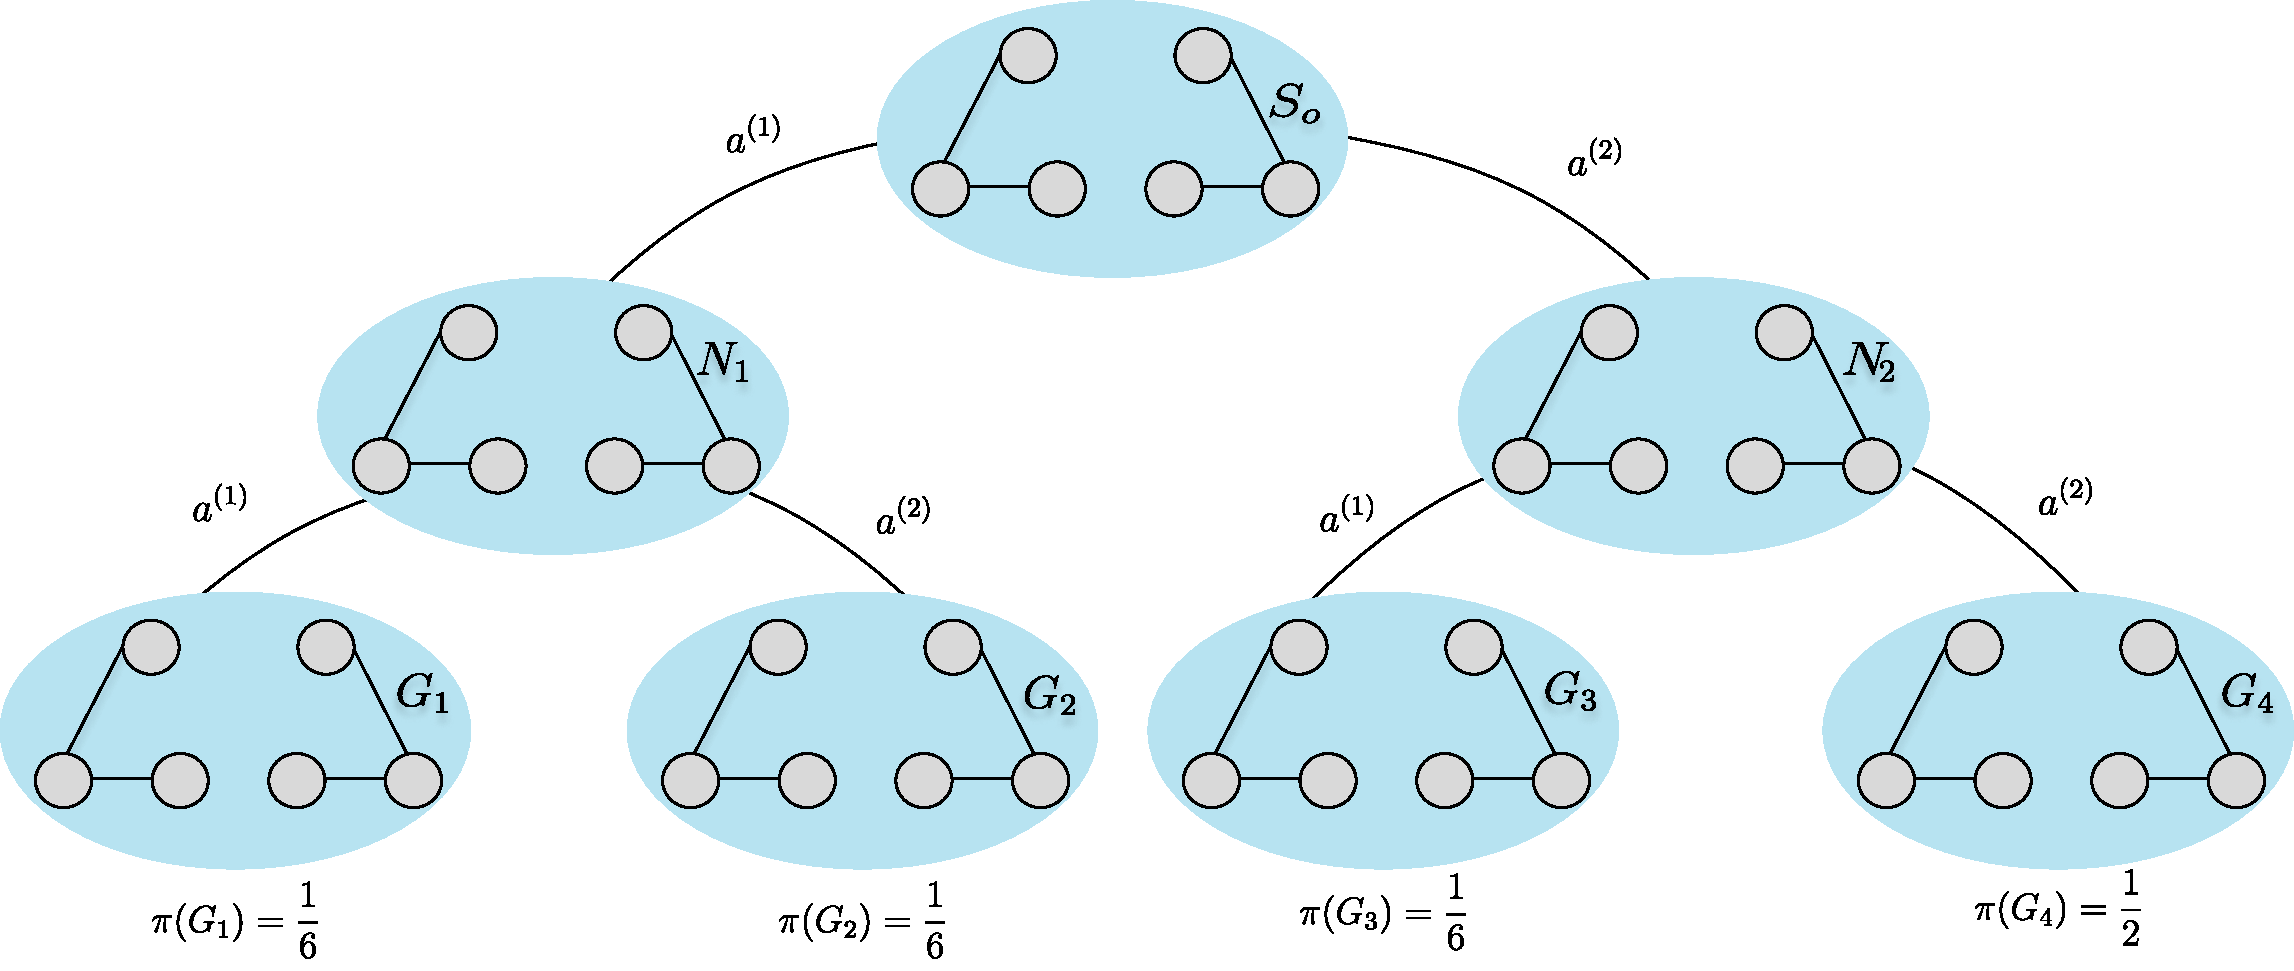
\includegraphics[scale=.3]{gflownets_wl_test.pdf} 
    \caption{A state graph whose downstream distribution is not learnable by a GFlowNet with a policy network is
    parametrized by a 1-WL GNN.} 
    \label{fig:wl_graphs} 
\end{figure}

\begin{theorem}[Distributional constraints of GFlowNets] 
    Let $\mathcal{G} = \{(\mathbf{X}, \mathbf{A}) \colon \mathbf{A} \in \{0,
    1\}^{N \times N}\}$ be the set of equally featured graphs with adjacency matrix $\mathbf{A}$
    and features $\mathbf{r} \in \mathbb{R}^{d}$ ($\mathbf{X} = \mathbf{1}\mathbf{r}^{T} \in \mathbb{R}^{N \times d}$). Let $F_{\theta} \colon \mathcal{G} \rightarrow \Delta_{2}$ be the
    \textit{policy network} that maps a graph $G \in \mathcal{G}$ to a point within the simplex of action-probabilities $\Delta_{2} =
    \{(a^{(1)}, a^{(2)}) \colon a^{(1)} + a^{(2)} = 1 \text{ and
    } a^{(1)}, a^{(2)} \ge 0\}$. See Figure~\ref{fig:wl_graphs}. Suppose that the policy network is parametrized by an 1-WL GNN with parameters $\theta$. Let $\pi$ be a distribution on the
    graphs $\{G_{i} \colon i \in \{1, 2, 3, 4\}\}$ of Figure~\ref{fig:wl_graphs} with $\pi(G_{1}) = \pi(G_{2}) = \pi(G_{3}) =
    \frac{1}{6}$ and $\pi(G_{4}) = \frac{1}{2}$. In these settings, there does not exist a
    $\theta$ such that the downstream distribution induced by the policy network equals $\pi$. 
\end{theorem}

\begin{proof}
    Let $p_{\theta}(X | S_{o})$ be the marginal transition probability learned by the GFlowNet of reaching the state $X
    \in \mathcal{G}$
    through the generative process characterized by the state graph of Figure~\ref{fig:wl_graphs} and the policy network
    $F_{\theta}$. We will show that
    $p_{\theta}(G_{i} | S_{o})$ is -- for any $\theta$ -- necessarily different of $\pi(G_{i})$ for at least two graphs
    in $\pi$'s support. 

    For this, notice that the Markovity of the stochastic transitions learned by the GFlowNet
    entails that 
    $p_{\theta}(G_{1} | S_{o}) = p_{\theta}(N_{1} | S_{o}) p_{\theta}(G_{1} | N_{1})$, 
    $p_{\theta}(G_{2} | S_{o}) = p_{\theta}(N_{1} | S_{o}) p_{\theta}(G_{2} | N_{1})$, 
    $p_{\theta}(G_{3} | S_{o}) = p_{\theta}(N_{2} | S_{o}) p_{\theta}(G_{3} | N_{2})$ and  
    $p_{\theta}(G_{4} | S_{o}) = p_{\theta}(N_{2} | S_{o}) p_{\theta}(G_{4} | N_{2})$. 
    Notably, the indistinguishability of the graphs $N_{1}$ and $N_{2}$ according to the 1-WL 
    isomorphism test implies that $F_{\theta}(N_{1}) = F_{\theta}(N_{2})$ and hence the transition  
    probabilities must satisfy $p_{\theta}(G_{1} | N_{1}) = p_{\theta}(G_{3} | N_{2})$ and $p_{\theta}(G_{2} | N_{1}) =
    p_{\theta}(G_{4} | N_{2})$. 

    Contradictorily, suppose that there is a $\theta$ such that the policy network $F_{\theta}$ is perfectly adjusted to the target distribution $\pi$.
    Hence, $p_{\theta}(G_{i} | S_{o}) = \pi(G_{i})$ for each $i \in \{1, 2, 3, 4\}$. Nonetheless, the representational equivalence of
    $N_{1}$ and $N_{2}$ and the Markovian assumption imply that 

    \begin{equation*} 
        \begin{split} 
        p_{\theta}(N_{1} | S_{o}) = \frac{\pi(G_{1})}{p_{\theta} (G_{1} | N_{1})} 
        = \frac{\pi(G_{3})}{p_{\theta} (G_{3} | N_{2})} = p_{\theta}(N_{2} | S_{o}) 
        \text{ and that } \\ 
        p_{\theta}(N_{1} | S_{o}) = \frac{\pi(G_{2})}{p_{\theta}(G_{2} | N_{1})} \neq 
        \frac{\pi(G_{4})}{p_{\theta}(G_{4} | N_{2})} = p_{\theta}(N_{2} | S_{o}).
        % p_{\theta}(N_{1} | S_{o}) = 
    \end{split} 
    \end{equation*} 

   \noindent This contradiction guarantees that $p(G_{i} | S_{o})$ is necessarily different from $\pi(G_{i})$ for at
   least a pair of graphs and asseverates that the distribution characterized by the state graph of
   Figure~\ref{fig:wl_graphs} is unlearnable by a GFlowNet parametrized by a 1-WL GNN. 
\end{proof}

\begin{remark}
    The previous theorem states the limitations of a GFlowNet parametrized by a 1-WL GNN. The alternative use of a more
    expressive yet not permutationally invariant flow parametrization would entail a factorially large increase of the
    size of the state graph, as equivalent graphs with different labelling would be treated differently by the flow
    estimator, and lead to a computationally untractable problem. The next theorem characterizes a weak relationship
    between the size of the state graph and the statistical efficiency of a maximally entropic exploratory policy within the state graph.   
\end{remark}

\subsubsection*{Author Contributions}
If you'd like to, you may include  a section for author contributions as is done
in many journals. This is optional and at the discretion of the authors.

\subsubsection*{Acknowledgments}
Use unnumbered third level headings for the acknowledgments. All
acknowledgments, including those to funding agencies, go at the end of the paper.
 

\appendix

% \section{Claimed Emergent Abilities}
% \label{app:claimed_emergent_abilities}

% We compile the models, tasks and metrics that different papers have claimed reveal emergent abilities of large language models. This list may be incomplete or inaccurate, but represents a good faith attempt to compile this information. Note: quantifying model scale when an ability emerges is complicated by the fact that different papers report model scale differently, either as (a) number of parameters \cite{brown2020language, ganguli2022predictability}, (b) effective number of parameters \cite{srivastava2022beyond} or (c) training FLOPs \cite{wei2022emergent}.

% \begin{table}[h!]
%     \centering
%     \begin{tabular}{|l|c|c|c|}
%     \hline
%         Task & Model Families & Metric & Model Scale at Emergence \\
%         \hline
%         2-Digit Addition \cite{brown2020language} & GPT-3 & Accuracy & 13B Parameters\\
%         2-Digit Subtraction \cite{brown2020language} & GPT-3 & Accuracy & 13B Parameters\\
%         3-Digit Addition \cite{brown2020language, ganguli2022predictability} & GPT-3 & Accuracy & 175B Parameters\\
%         3-Digit Subtraction \cite{brown2020language} & GPT-3 & Accuracy & 175B Parameters\\
%         MMLU \cite{ganguli2022predictability} & GPT-3, Gopher & Accuracy & 200B, 300B Parameters\\
%         Program Synthesis \cite{ganguli2022predictability} & Google Internal & \% Samples Solving Task & 200B Parameters\\
%         Figure of Speech Detection \cite{srivastava2022beyond} & ? & ? & $\sim 10^{11}$ Effective Parameters \\
%         IPA Transliterate \cite{srivastava2022beyond, wei2022emergent} & LaMDA, GPT-3 & BLEU & $\sim 10^{23}, \sim 10^{23}$ Training FLOPs\\
%         Periodic Elements \cite{srivastava2022beyond} & ? & ? & ?\\
%         Modified Arithmetic \cite{srivastava2022beyond, wei2022emergent} & GPT-3, LaMDA & Accuracy & $\sim 10^{23}, \sim 10^{24}$ Training FLOPs\\
%         Repeat Copy Logic \cite{srivastava2022beyond} & ? & ? & $10^{11}$ Effective Parameters\\
%         Word Unscrambling \cite{srivastava2022beyond, wei2022emergent} & LaMDA & Exact Match & $\sim 10^{24}$ Training FLOPs\\
%         Persian QA \cite{wei2022emergent} & PaLM & Exact Match & $\sim 10^{24}$ Training FLOPs\\
%         Truthful QA \cite{wei2022emergent} & Gopher & Accuracy & $\sim 10^{23}$ Training FLOPs\\
%         Grounded Mappings \cite{wei2022emergent} & ? & ? & ?\\
%         Multi-task NLU \cite{wei2022emergent} & ? & ? & ?\\
%         Word in context \cite{wei2022emergent} & ? & ? & $\sim 10^{24}$ Training FLOPs\\
%         \hline
%     \end{tabular}
%     \newline
%     \caption{\textbf{Tasks, model families, metrics and number of parameters for emergent abilities.}}
%     \label{tab:my_label}
% \end{table}


% \section{Exponentiated Negative Cross Entropy Lower Bounds Accuracy}
% \label{app:acc_bound}

% Consider batch size $B$ with length $L$. During training i.e. with teacher-forcing, the per-token accuracy (averaged over batch index $b$ and sequence index $l$) is defined as:
% %
% \begin{align}
%     \text{Acc} &\defeq \frac{1}{B} \sum_b \frac{1}{L} \sum_l p(t_{bl}^* | t_{b, <l}^*)\\
%     &= \frac{1}{BL} \sum_{b, l} p(t_{bl}^* | t_{b, <l}^*)
% \end{align}

% The cross entropy (commonly averaged over the batch) is defined as:
% %
% \begin{align}
%     \mathcal{L}_{CE} &\defeq -\frac{1}{B} \sum_b \log p(t_{b 1}^*, ..., t_{b L}^*)\\
%     &= -\frac{1}{B} \sum_b \log \prod_l p(t_{b l}^*| t_{b, <l}^*)\\
%     &= -\frac{1}{B} \sum_{b, l} \log p(t_{bl}^* | t_{b, <l}^*)
% \end{align}

% To make the comparison between accuracy and cross entropy a little easier, let's normalize the cross entropy by the sequence length:
% %
% \begin{align}
%     \mathcal{L}_{CE/L} &\defeq \frac{1}{L}\mathcal{L}_{CE}\\
%     &=  -\frac{1}{BL} \sum_{b, l} \log p(t_{bl}^* | t_{b, <l}^*)
% \end{align}

% Recall that Jensen's inequality tells us that for any random variable $X$, $\log \mathbb{E}[X] \geq \mathbb{E}[\log X]$. The relationship between sequence-length-normalized cross entropy and accuracy is thus:
% %
% \begin{align}
%     -\mathcal{L}_{CE/L} = \frac{1}{BL} \sum_{b, l} \log p(t_{bl}^* | t_{b <l}^*) &\leq \log \frac{1}{BL} \sum_{b, l}  p(t_{bl}^* | t_{b <l}^*) = \log \text{Acc}\\
%     \exp(- \mathcal{L}_{CE/L}) &\leq \text{Acc}
% \end{align}

% Consequently, we see that driving the cross entropy loss to $0$ necessarily drives the accuracy to $1$.

% TODO: Can we use the second moment method to derive bounds on how (un)likely a subset of tokens are to deviate from the mean?


\section{Approximate Behavior of Metrics on Sequential Data}
\label{app:metric_scaling}

How do different metrics behave when used to measure autoregressive model outputs? Precisely answering this question is tricky and possibly analytically unsolvable, so we provide an approximate answer here.

Notationally, we consider $N$ test data of length $L$ (here, length is measured in tokens) with targets denoted $t_n \defeq (t_{n1}, t_{n2}, ... t_{nL})$, the autoregressive model has a true-but-unknown per-token error probability of $\epsilon \in [0, 1]$ and the model outputs prediction $\hat{t}_n \defeq (\hat{t}_{n1}, \hat{t}_{n2}, ... \hat{t}_{nL})$. This assumes that the model's per-token error probability is constant, which is empirically false, but modeling the complex dependencies of errors is beyond our scope.

\subsection{Per-Token Error Probability is Resolution-Limited}
\label{app:metric_scaling:resolution_limited}

Note that because we have $N$ test data, each of length $L$, our resolution for viewing the per-token error probability $\epsilon$ is limited by $1/NL$. 
Here, resolution refers to ``the smallest interval measurable by a scientific instrument; the resolving power."
To explain what resolution means via an example, suppose one wants to measure a coin's probability of yielding heads.
After a single coin flip, only two outcomes are possible (H, T), so the resolution-limited probability of heads is either $0$ or $1$.
After two coin flips, four outcomes are possible (HH, HT, TH, TT), so the resolution-limited probability of heads is now one of $0, 0.5, 1$.
After $F$ coin flips, we can only resolve the coin's probability of yielding heads up to $1/F$.
Consequently, we introduce a resolution-limited notation:
%
\begin{equation}
    \nint{a}_b \defeq \text{$a$ rounded to the nearest integer multiple of $1/b$}
\end{equation}

\subsection{Token Edit Distance}
\label{app:metric_scaling:token_edit_distance}

We first consider an adaptation of the Levenshtein (string edit) distance for models that function on tokens rather than characters, an adaptation we term the \textit{token edit distance}. The token edit distance between two token sequences $t_n, \hat{t_n}$ is defined as the integer number of additions, deletions or substitutions necessary to transform $t_n$ into $\hat{t}_n$ (or vice versa).

\begin{align}
    \text{Token Edit Distance}(t_n, \hat{t}_n)  &\defeq \text{Num Substitutions} + \text{Num. Additions} + \text{Num. Deletions}\\
    &= \sum_{\ell =1}^L \mathbb{I}[t_{n\ell} \neq \hat{t}_{n\ell}] + \text{Num. Additions} + \text{Num. Deletions}\\
    &\geq \sum_{\ell =1}^L \mathbb{I}[t_{n\ell} \neq \hat{t}_{n\ell}]
\end{align}

The expected token edit distance is therefore:

\begin{align}
    \mathbb{E}[\text{Token Edit Distance}(t_n, \hat{t}_n)] &\geq \mathbb{E}[\sum_{\ell =1}^L \mathbb{I}[t_{n\ell} \neq \hat{t}_{n\ell}]]\\
    &= \sum_{\ell =1}^L p(t_{n\ell} \neq \hat{t}_{n\ell})\\
    &\approx L (1 - \epsilon)
\end{align}

The resolution-limited expected token edit distance is therefore:

\begin{equation}
    \nint{\mathbb{E}[\text{Token Edit Distance}(t_n, \hat{t}_n)]}_{NL} \geq L \Big(1 - \nint{\epsilon}_{NL} \Big)
\end{equation}

From this, we see that the expected token edit distance scales approximately linearly with the resolution-limited per-token probability. The real rate is slightly higher than linear because additions and deletions contribute an additional non-negative cost, but modeling this requires a model of how likely the model is to overproduce or underproduce tokens, which is something we do not currently possess.

\subsection{Accuracy}
\label{app:metric_scaling:accuracy}

\begin{align}
    \text{Accuracy}(t_n, \hat{t}_n) &\defeq \mathbb{I}[\text{No additions}] \, \mathbb{I}[\text{No deletions}] \, \prod_{l=1}^L \mathbb{I}[t_{nl} = \hat{t}_{nl}]\\
    &\approx \prod_{l=1}^L \mathbb{I}[t_{nl} = \hat{t}_{nl}]
\end{align}

As with the Token Edit Distance (App. \ref{app:metric_scaling:accuracy}), we ignore how likely the language model is to overproduce or underproduce tokens because we do not have a good model of this process. Continuing along,

\begin{align}
    \mathbb{E}[\log \text{Accuracy}] &= \sum_l \mathbb{E}[\log \mathbb{I}[t_{nl} = \hat{t}_{nl}]]\\
    &\leq \sum_l \log \mathbb{E}[\mathbb{I}[t_{nl} = \hat{t}_{nl}]]\\
    &\approx L \log (1- \epsilon)
    % \exp(\mathbb{E}[\log \text{Accuracy}]) &= \exp (\sum_l \mathbb{E}[\log \mathbb{I}(t_{nl}, \hat{t}_{nl})])\\
    % &=
\end{align}

Taking an approximation that would make most mathematicians cry:

\begin{align}
    \mathbb{E}[\text{Accuracy}] &\approx \exp(\mathbb{E}[\log \text{Accuracy}])\\
    &= (1 - \epsilon)^L\\
\end{align}

This reveals that accuracy \textbf{approximately} falls geometrically with target token length. The resolution-limited expected accuracy is therefore:

\begin{equation}
    \nint{\mathbb{E}[\text{Accuracy}]}_{NL} = \nint{(1 - \epsilon)^L}_{NL}
\end{equation}

From this we can see that choosing a nonlinear metric like Accuracy is affected significantly more by limited resolution because Accuracy forces one to distinguish quantities that decay rapidly.

\subsection{ROUGE-L-Sum}
\label{app:metric_scaling:rougeLsum}

\begin{figure}
    \centering
    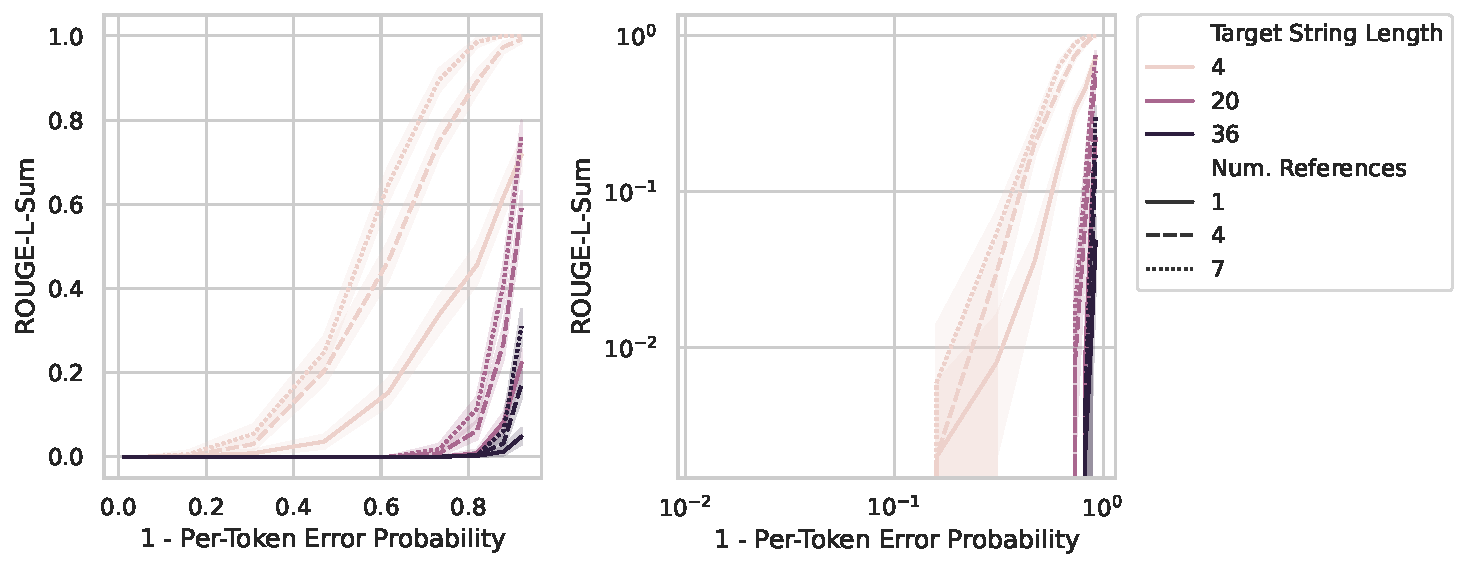
\includegraphics[width=0.95\textwidth]{figures/rouge_understanding/rougeLsum_vs_token_error_prob_scaling_simulation.pdf}
    \caption{\textbf{ROUGE-L-Sum is a sharp metric.} Simulations show that as the per-token error probability slightly increase (e.g. from 0.05 to 0.1), the ROUGE-L-Sum metric sharply falls.}
    \label{fig:app:metric_scaling:rougeLsum}
\end{figure}


Another BIG-Bench metric \cite{srivastava2022beyond} is ROUGE-L-Sum \cite{lin2004rouge}, a metric based on the longest common subsequence (LCS) between two sequences. Section 3.2 of \cite{lin2004rouge} gives the exact definition, but the key property is that ROUGE-L-Sum measures the ``union" LCS, which means ``stitching" together LCSs across the candidate and multiple references. As explained in the original paper: if the candidate sequence is $c = w_1 w_2 w_3 w_4 w_5$, and if there are two reference sequences $r_1 = w_1 w_2 w_6 w_7 w_8$ and $r_2 = w_1 w_3 w_8 w_9 w_5$, then $LCS(r_1, c) = w_1 w_2$ and $LCS(r_2, c) =w_1 w_3 w_5$, then the \textit{union} 
-LCS of $c, r_1, r_2$ is $w_1 w_2 w_3 w_5$, with length 4. Intuitively, this disproportionately benefits models with smaller error rates because their mistakes can be ``stitched" across multiple references; this is confirmed in simulation (Fig. \ref{fig:app:metric_scaling:rougeLsum}).


% \subsection{BLEU}
% \label{app:metric_scaling:bleu}


% \subsection{Emergence does not require on scaling laws: decreasing cross-entropy loss and stricter exact match is all you need }

% The goal of this section is to show that scaling laws are not necessary to create emergence and that many functional forms of the loss are valid as long as the form decreases as some other variable decreases -- say the number of parameters in the model.
% This typically holds in modern machine learning. 
% We do this by considering different functional forms of the cross entropy $CE(N)$, as a function of the number of parameters $N$, and show emergence, i.e. sharpness and unpredictability.
% We illustrate this by showing the programmer can exaggerate the sharpness (and therefore emergence) by implying increasing the exact number of tokens required to get correct in the accuracy, i.e. increasing $L$ in our notation.

% \subsubsection{Argument}

% Recall from section \ref{sec:alt_explanation} the accuracy requiring all $L$ tokens to be correct for a model of size $N$ as a function of cross-entropy $CE(N)$:

% \begin{equation*}
%     \text{Accuracy}(N) \approx p_N(\text{single token correct})^{\text{num. of tokens}} = \exp \Big(- CE(N) \Big)^L
% \end{equation*}

% We plot this equation using three functional forms for a decreasing cross-entropy loss in figure \ref{fig:decreasing_loss_leads_to_emergence_as_L_increases} for increasing values of $L$.
% These increasing values of $L$ induce a sharper -- therefore, seemingly more emergent curve when plotting the accuracy. 
% This means that if the programmer simply requires a stricter accuracy, he can make a perfectly smooth and predictable cross-entropy loss suddenly become sharp and unpredictable, i.e. ``emergent". 
% We show numerically it is independent of the functional form and instead that it only requires the cross-entropy to be decreasing and the accuracy metric to have some non-linear transformation that makes it sharper. 
% Therefore, if one had only tracked the cross-entropy loss instead, one could have had a smooth predictable curve for the models.
% This implies small-scale experimentation is still relevant, and we wish to highly that GPT-4 \cite{gpt4} small-scale experiment in conjunction with scaling loss. 
% We'd like to emphasize that changing the evaluation metric can suddenly induce emergence, and it is not an intrinsic property of the model. 

% %The goal will be to show that if $CE(N)$ decreases with different functional forms that $acc$ is emergent (either sharp or unpredictable).
% % TODO: sharp due to L
% % TODO: unpredictable due to constant and L

% \begin{figure}[htbp]
%   \centering
%   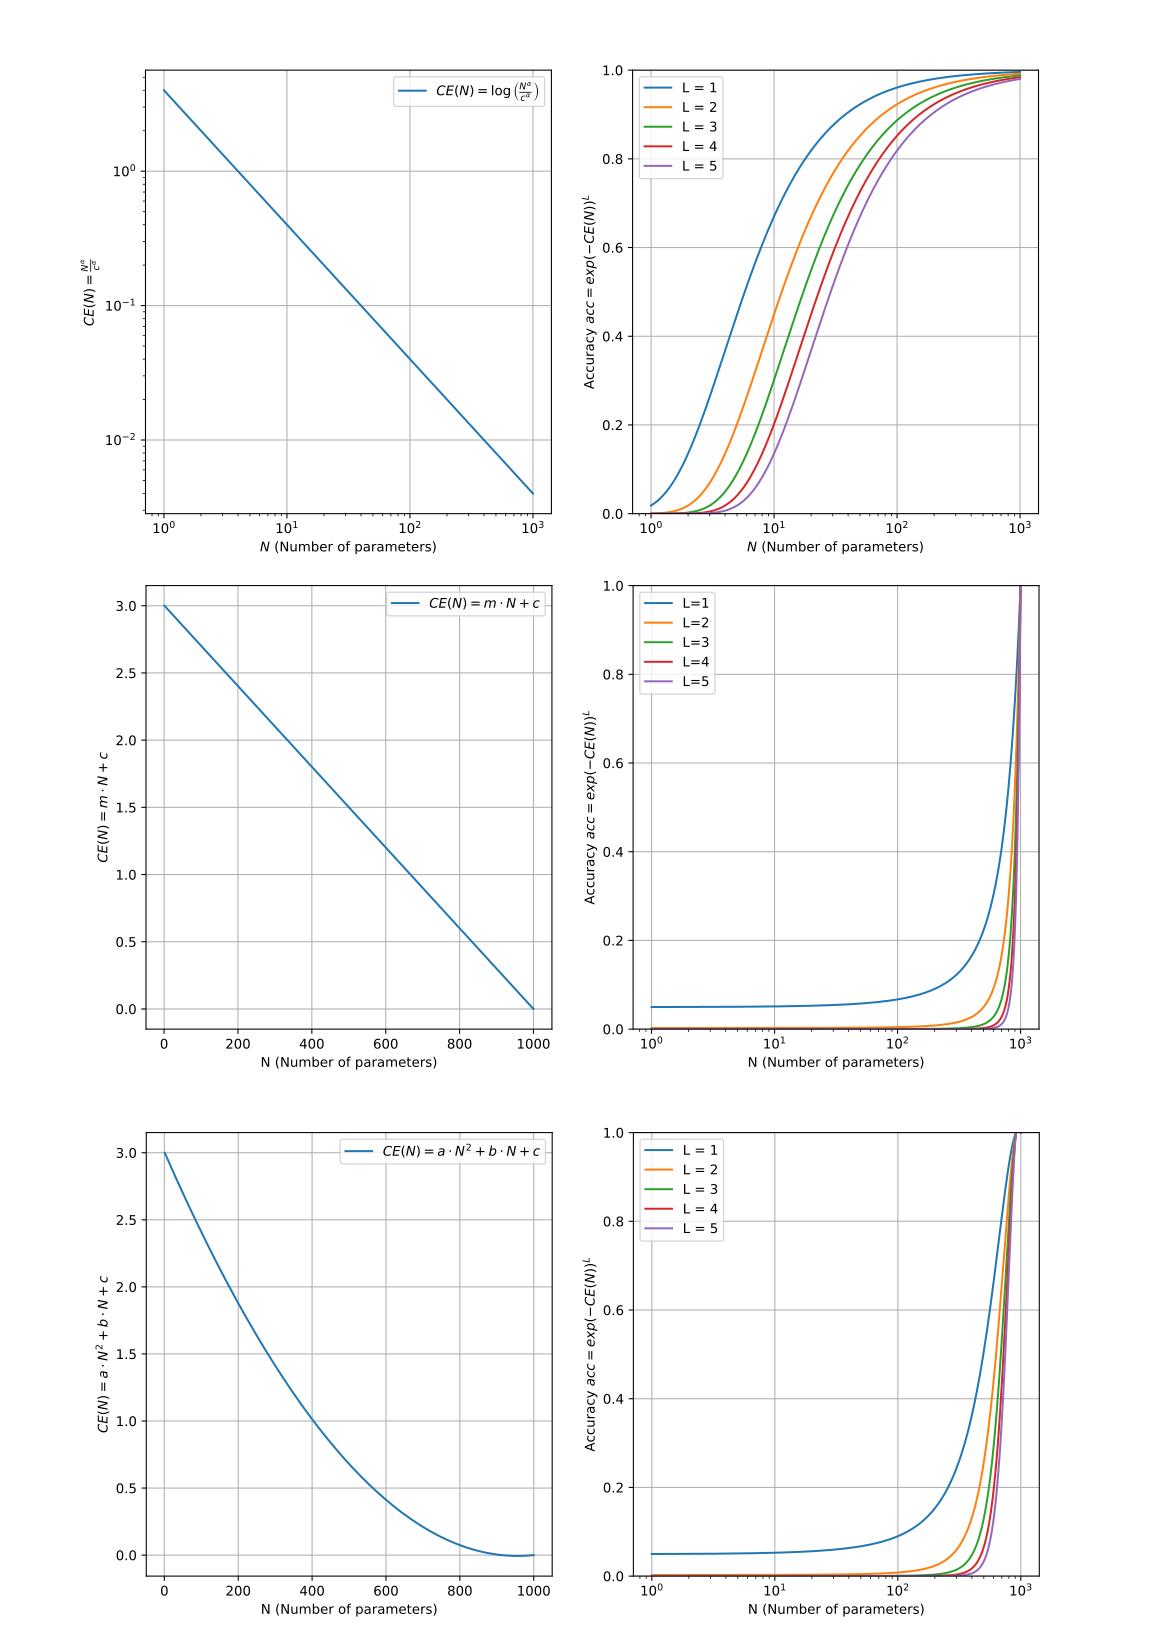
\includegraphics[width=0.8\textwidth]{figures/loss_decreasing_leads_to_emergence/decreasing_loss_leads_to_emergence_as_L_increases.png}
%   \caption{
%   \textbf{Emergence does not depend on scaling laws: any decreasing cross-entropy loss induces apparent emergence as L increases as you require more tokens to be exactly correct, i.e. L increases.}
%   The first row shows the same argument as in the main section, where a decreasing cross-entropy loss as a scaling law induces emergence as $L$ increases.
%   The second row shows the that apparent emergence is induced even when the cross-entropy loss decreases linearly.
%   The third row shows that the apparent emergence is induced when the cross-entropy loss decreases quadratically.
%   Emergence is amplified in this case especially by the increase in sharpness as more tokens are required to be correct. 
%   This means that simply changing the evaluation metric can suddenly induce emergence, and it is not an intrinsic property of the model. 
%   }
%   \label{fig:decreasing_loss_leads_to_emergence_as_L_increases}
% \end{figure}


\section{Inducing Emergent Abilities in Networks on Vision Tasks}
\label{app:sec:inducing_emergence_vision}

\subsection{Emergent Classification of MNIST Handwritten Digits by Convolutional Networks}

\begin{figure}
    \centering
    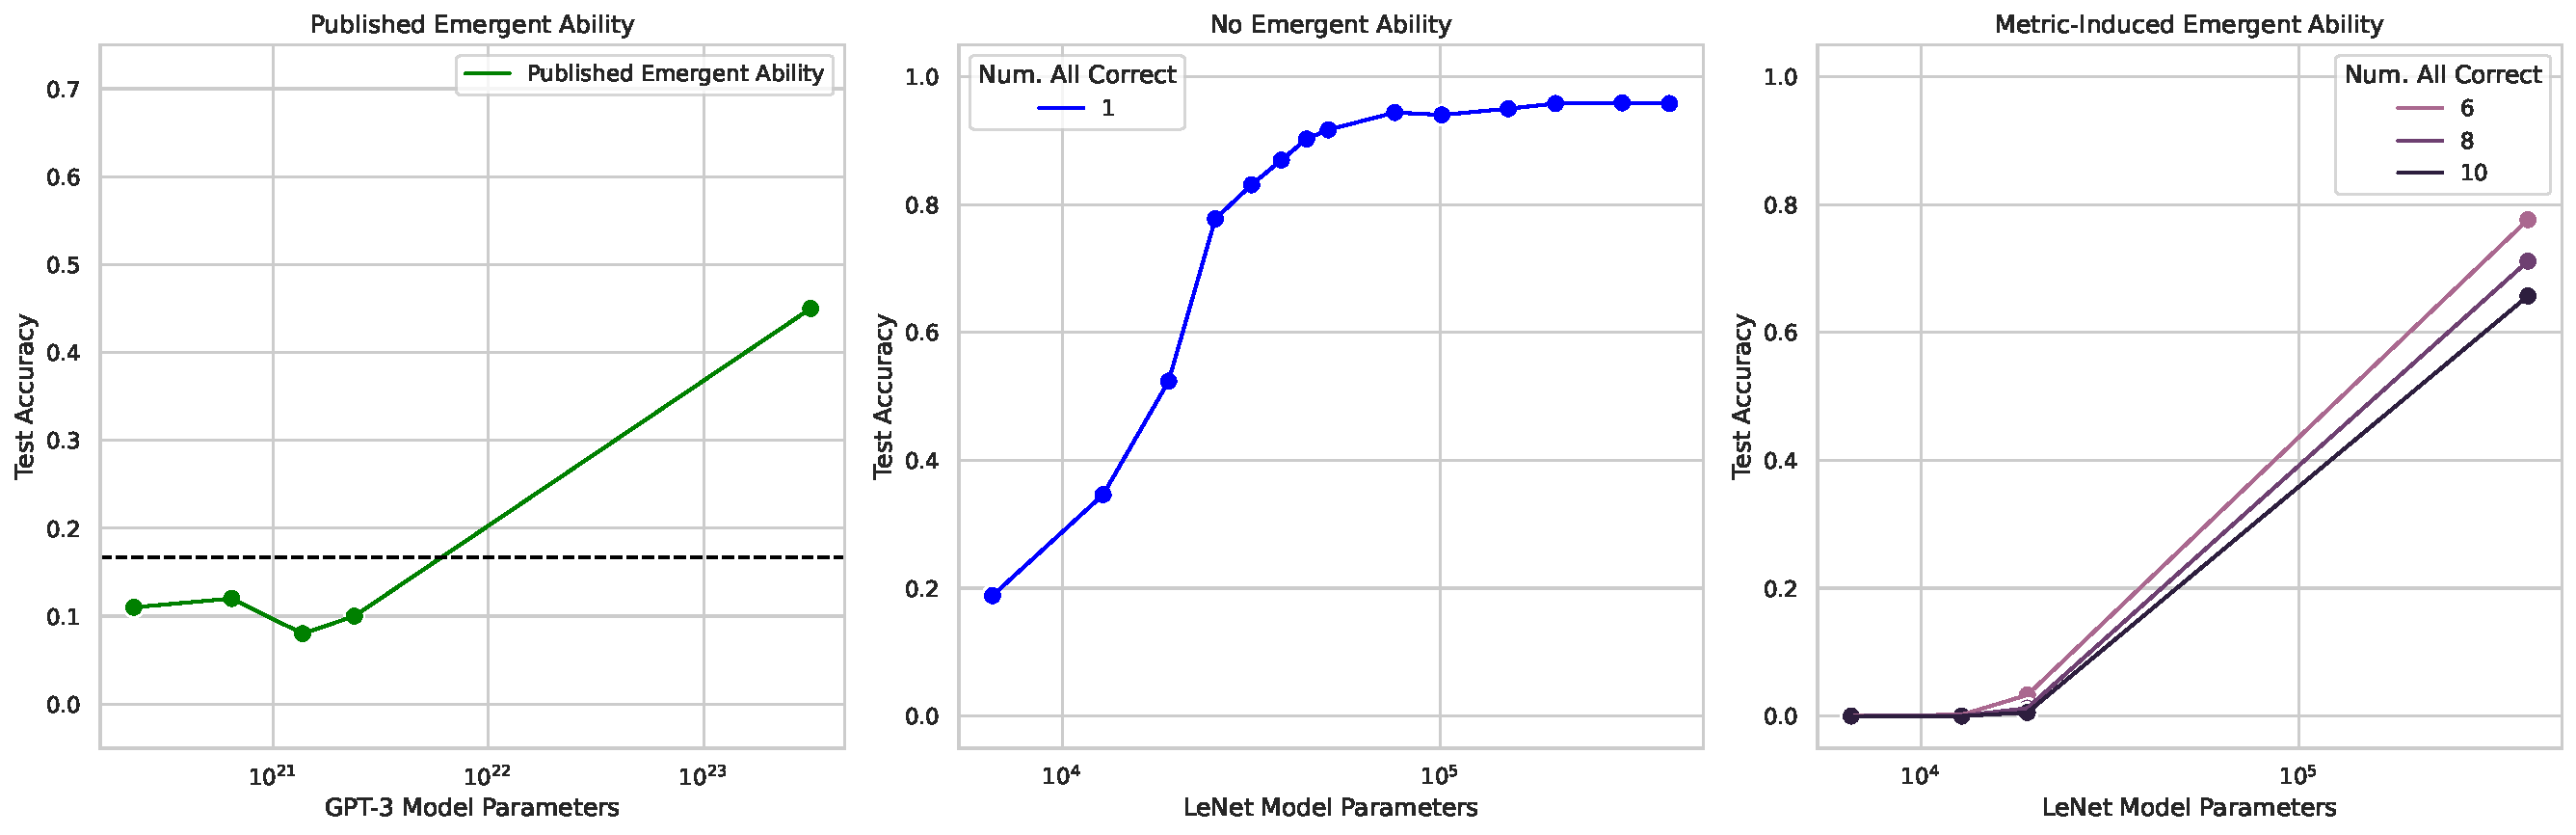
\includegraphics[width=\textwidth]{figures/vision/no_emergence_and_emergence_dataset=mnist.pdf}
    \caption{\textbf{Induced emergent MNIST classification ability in convolutional networks.} (A) A published emergent ability from the BIG-Bench Grounded Mappings task \cite{wei2022emergent}. (B) LeNet trained on MNIST \cite{lecun1998mnist} displays a predictable, commonplace sigmoidal increase in test accuracy as model parameters increase. (C) When accuracy is redefined as correctly classifying $K$ out of $K$ independent test data, this newly defined metric induces a seemingly unpredictable change.}
    \label{fig:vision_mnist}
\end{figure}

We begin by inducing an emergent classification ability in a LeNet convolutional neural network family \cite{lecun1998gradient}, trained on the MNIST handwritten digits dataset \cite{lecun1998mnist}.
This family displays smoothly increasing test accuracy as the number of parameters increase (Fig. \ref{fig:vision_mnist}B).
To emulate the accuracy metric used by emergence papers \cite{ganguli2022predictability, wei2022emergent, srivastava2022beyond}, we use \textit{subset accuracy}: 1 if the network classifies $K$ out of $K$ (independent) test data correctly, 0 otherwise.
Under this definition of accuracy, the model family displays an ``emergent" ability to correctly classify sets of MNIST digits as $K$ increases from $1$ to $5$, especially when combined with sparse sampling of model sizes (Fig. \ref{fig:vision_mnist}C).
This convolutional family's emergent classification ability qualitatively matches published emergent abilities, e.g., at the BIG-Bench Grounded Mappings task \cite{wei2022emergent} (Fig. \ref{fig:vision_mnist}A).
 


\end{document}


% This document was modified from the file originally made available by
% Pat Langley and Andrea Danyluk for ICML-2K. This version was created
% by Iain Murray in 2018, and modified by Alexandre Bouchard in
% 2019 and 2021 and by Csaba Szepesvari, Gang Niu and Sivan Sabato in 2022.
% Modified again in 2023 and 2024 by Sivan Sabato and Jonathan Scarlett.
% Previous contributors include Dan Roy, Lise Getoor and Tobias
% Scheffer, which was slightly modified from the 2010 version by
% Thorsten Joachims & Johannes Fuernkranz, slightly modified from the
% 2009 version by Kiri Wagstaff and Sam Roweis's 2008 version, which is
% slightly modified from Prasad Tadepalli's 2007 version which is a
% lightly changed version of the previous year's version by Andrew
% Moore, which was in turn edited from those of Kristian Kersting and
% Codrina Lauth. Alex Smola contributed to the algorithmic style files.
